\ifdefined\ishandout
\documentclass[handout]{beamer}
\else
\documentclass{beamer}
\fi

%\usepackage[frenchb]{babel}
\usepackage[T1]{fontenc}
%\usepackage[utf8]{inputenc}
\usepackage{hyperref}
\usepackage{multirow}
\usepackage{listings}
\usepackage{rotating}

\usepackage{fancyvrb}
\usepackage{tikz}
\usepackage{framed}
\usepackage{algorithm}
\usepackage{algorithmic}
\usepackage{xcolor}
\usepackage{booktabs}
\usepackage{color, colortbl}
\ifdefined\ishandout
\usepackage{handoutWithNotes}
\fi
\usepackage{slashbox}
\usepackage{amsmath}
\usepackage{bm}
\usepackage{hhline}
\usepackage{pgfplots}
\usepackage{caption}
\usepackage{natbib}
\def\bibfont{\footnotesize}
\def\bibname{}


\usetikzlibrary{shapes.geometric}
\usetikzlibrary{positioning}
\usetikzlibrary{shapes.arrows, chains}
\usetikzlibrary{arrows,calc}
\usetikzlibrary{shapes.multipart}
\usetikzlibrary{matrix}
\usetikzlibrary{fit}

\usepackage{array}
%\usetheme{Boadilla}
\usetheme[progressbar=frametitle]{metropolis}

\usefonttheme[onlymath]{serif}

\newcommand{\R}{\mathbb{R}}
%\newcommand{\C}{\mathbb{C}}
\newcommand{\N}{\mathbb{N}}
\newcommand{\Z}{\mathbb{Z}}
\newcommand{\E}{\mathbb{E}}
\newcommand{\Var}{\text{Var}}
\newcommand{\Cov}{\text{Cov}}

\newcommand{\btheta}{\mathbf{\theta}}
\newcommand{\M}{\mathcal{M}}


\ifdefined\ishandout
\pgfpagesuselayout{3 on 1 with notes}[a4paper,border shrink=5mm]
\usecolortheme{dove}
\else
%\usecolortheme{dolphin}
%\usecolortheme{crane}
\fi

\metroset{block=fill}

\lstnewenvironment{codeC}
{ \lstset{language=C,
    otherkeywords={printf,scanf}}
}
{}

\ifdefined\ishandout
\definecolor{mygreen}{rgb}{0,0,0}
\definecolor{mymauve}{rgb}{0,0,0}
\definecolor{myblue}{rgb}{0,0,0}
\else
\definecolor{mygreen}{rgb}{0,0.6,0}
\definecolor{mymauve}{rgb}{0.58,0,0.82}
\definecolor{myblue}{rgb}{0,0,1}

\fi

%% Notes
%\setbeameroption{show only notes}


\definecolor{mygray}{rgb}{0.5,0.5,0.5}

\lstset{ language=Python,%
  backgroundcolor=\color{white},   % choose the background color; you must add \usepackage{color} or \usepackage{xcolor}
  basicstyle=\footnotesize,        % the size of the fonts that are used for the code
  breakatwhitespace=false,         % sets if automatic breaks should only happen at whitespace
  breaklines=true,                 % sets automatic line breaking
  captionpos=b,                    % sets the caption-position to bottom
  commentstyle=\color{mygreen},    % comment style
  deletekeywords={...},            % if you want to delete keywords from the given language
  escapeinside={\%*}{*)},          % if you want to add LaTeX within your code
  extendedchars=true,              % lets you use non-ASCII characters; for 8-bits encodings only, does not work with UTF-8
  frame=tb,	                   % adds a frame around the code
  keepspaces=true,                 % keeps spaces in text, useful for keeping indentation of code (possibly needs columns=flexible)
  keywordstyle=\color{blue},       % keyword style
  otherkeywords={*,...},           % if you want to add more keywords to the set
  numbers=none,                    % where to put the line-numbers; possible values are (none, left, right)
  numbersep=5pt,                   % how far the line-numbers are from the code
  numberstyle=\tiny\color{mygray}, % the style that is used for the line-numbers
  rulecolor=\color{black},         % if not set, the frame-color may be changed on line-breaks within not-black text (e.g. comments (green here))
  showspaces=false,                % show spaces everywhere adding particular underscores; it overrides 'showstringspaces'
  showstringspaces=false,          % underline spaces within strings only
  showtabs=false,                  % show tabs within strings adding particular underscores
  stepnumber=2,                    % the step between two line-numbers. If it's 1, each line will be numbered
  stringstyle=\color{mymauve},     % string literal style
  tabsize=3,	                   % sets default tabsize to 2 spaces
  title=\lstname                   % show the filename of files included with \lstinputlisting; also try caption instead of title
}
%\lstset{language=Python,
% breakatwhitespace=false,         % sets if automatic breaks should only happen at whitespace
%  breaklines=true,                 % sets automatic line breaking
%  captionpos=b,                
%%commentstyle=\itshape\color{mymauve},
%%keywordstyle=\bfseries\color{myblue},
%numbers=left,                    % where to put the line-numbers; possible values are (none, left, right)
%  numbersep=8pt,                   % how far the line-numbers are from the code
%  numberstyle=\tiny\color{mygray}, % the style that is used for the line-numbers
%%  rulecolor=\color{black},         % if not set, the frame-color may be changed on line-breaks within not-black text (e.g. comments (green here))
%  showspaces=false,                % show spaces everywhere adding particular underscores; it overrides 'showstringspaces'
%%  showstringspaces=false,          % underline spaces within strings only
%  showtabs=false,                  % show tabs within strings adding particular underscores
%  stepnumber=2,                    % the step between two line-numbers. If it's 1, each line will be numbered
%%  stringstyle=\color{mygreen},     % string literal style
%  tabsize=2 
%}
\ifdefined\ishandout
\newcommand{\red}{\textbf}
\else
\newcommand{\red}{\textcolor{red}}
\fi
%\newcommand \emph
%Default size : 12.8 cm * 9.6 cm

\newcommand{\tmark}[1]{\tikz[remember picture, baseline=-.5ex]{\coordinate(#1);}}

\definecolor{bluegreen}{RGB}{0,149,182}


%\newcommand{\output}[1]{
\setbeamertemplate{navigation symbols}{}
\newcommand{\bvrb}{\Verb[commandchars=£µ§,formatcom=\color{bluegreen}]}
\newcommand{\footvrb}{\footnotesize\Verb}
\newcommand{\vrbalert}[2][]{\visible<#1>{#2}}
%%% Commande pour les listes/arbres
\newcommand{\mvide}{\nodepart{one} \nodepart{two}}
\newcommand{\tvide}{\nodepart{one} \nodepart{two} \nodepart{three}}
\newcommand{\rref}[1][]{\hfill{\scriptsize\textit{#1}}}

%%Fin des commandes pour les listes/arbres.

\bibliographystyle{apalike}

%%% Paramètres du cours (à régler)
%Numéro du cours
\newcommand{\nb}{1}

\title[Machine Learning]{Machine learning and physical modelling-3}
\author[J. Brajard]{julien.brajard@nersc.no}
\institute[NERSC/SU]{NERSC/Sorbonne University\\
\url{https://github.com/brajard/Geilo-Winter-school}}
\date{21-25 January 2018}
\begin{document}
%%%%%%%%%%%%%%%%%%%%% SLIDES DE TITRE
\begin{frame}
\titlepage
%\centering{
%\url{http://australe.upmc.fr} (onglet EPU-C5-IGE Info Gen)}
\end{frame}

\begin{frame}{AI Art?}
    \begin{figure}
        \centering
        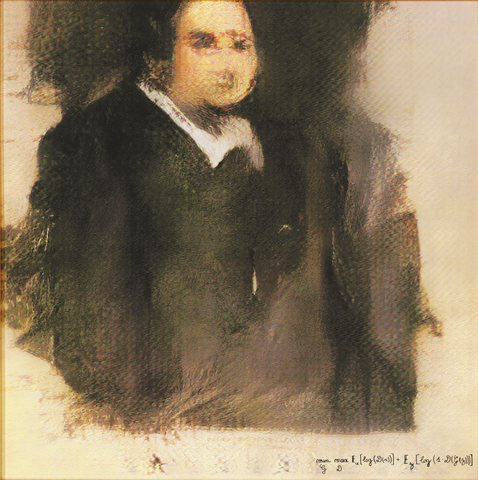
\includegraphics[width=0.5\textwidth]{fig/L3/478px-Edmond_de_Belamy.png}
        \caption*{\textit{Edmond de Bellamy} by Obvious(collective)}
    \end{figure}
    Generated using a Generative Adversarial Network.\\
    Selling prince (Oct. 2018): \$432,000
\end{frame}

\begin{frame}{Table of contents}
  \setbeamertemplate{section in toc}[sections numbered]
  \tableofcontents[hideallsubsections]
\end{frame}

\section{Machine learning to reveal complex connexions}
\begin{frame}{Altimeter data}
\begin{columns}[t]
\column{.5\textwidth}
    \begin{figure}
        \centering
        \caption*{Satellite altimeter}
         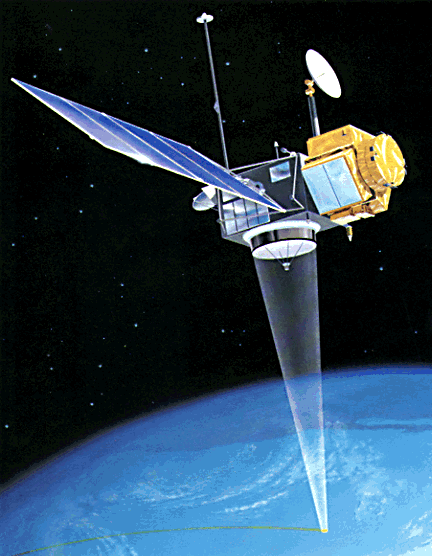
\includegraphics[width=.6\textwidth]{fig/L3/TOPEX-Poseidon.png}
    \end{figure}
    

\column{.5\textwidth}
    \begin{figure}
        \centering
        \caption*{Sea surface height anomaly}
         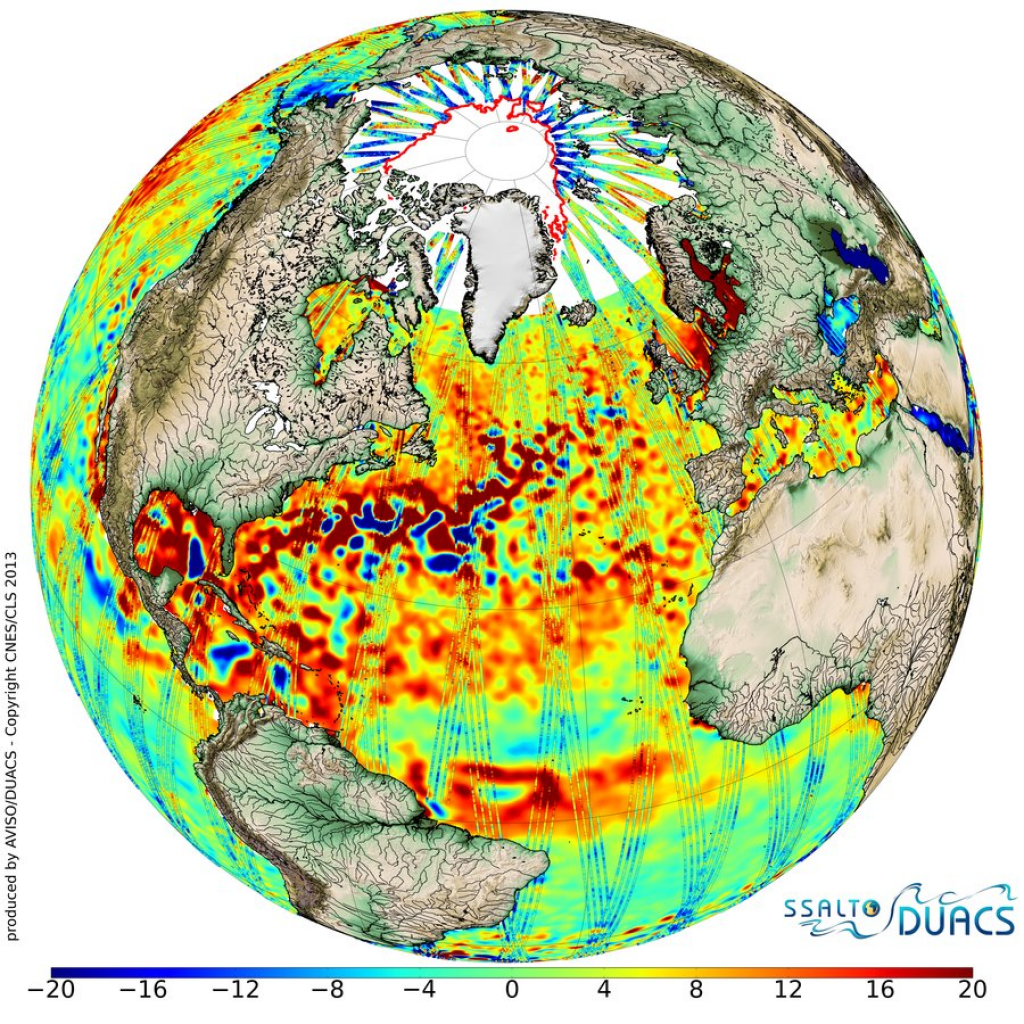
\includegraphics[width=.9\textwidth]{fig/L3/eddies.png}
    \end{figure}

    \end{columns}
    \begin{block}{Structure detection}
    Can we detect and charaterize eddies?
    \end{block}
\end{frame}

\begin{frame}[t]{Eddy detection}
\rref[\cite{Lguensat2017}]
    \begin{columns}
    \column{.65\textwidth}
     \begin{figure}
        \centering
         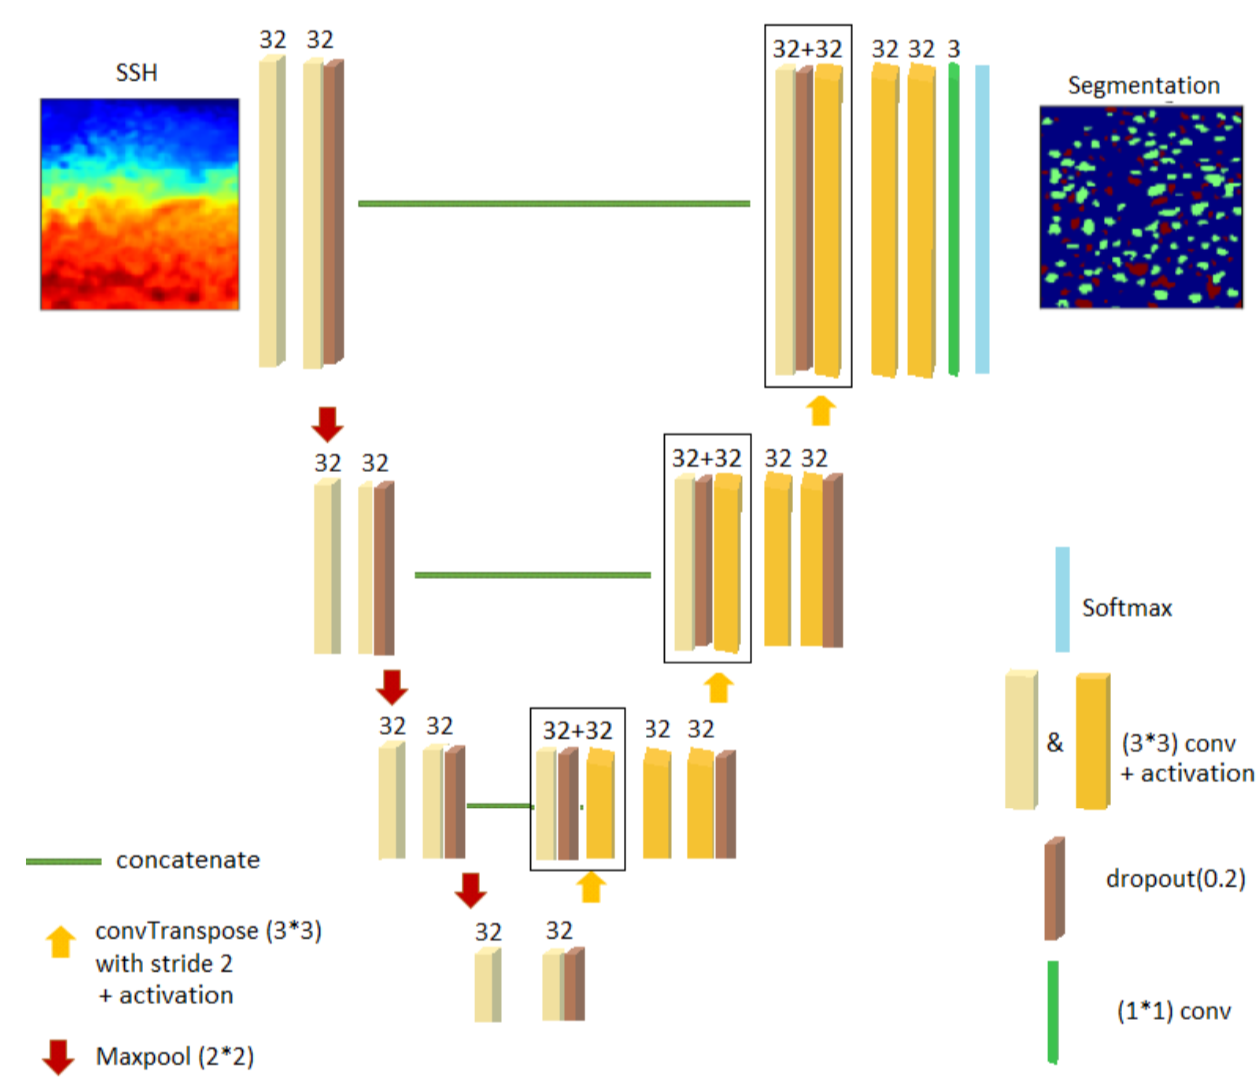
\includegraphics[width=\textwidth]{fig/L3/eddynet.png}
    \end{figure}

    \pause
    \column{.35\textwidth}
         \begin{figure}
        \centering
         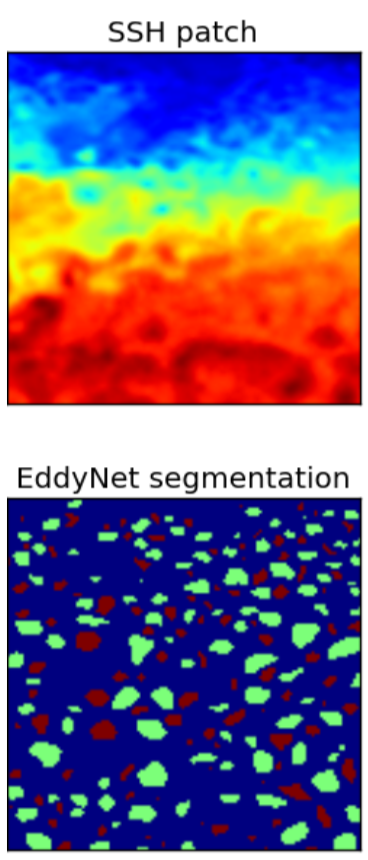
\includegraphics[width=.7\textwidth]{fig/L3/eddynet-result.png}
    \end{figure}
    \end{columns}
\end{frame}

\begin{frame}{Observations of sea velocity}
    %From Sea Surface Height (SSH) it is also possible to derive (partially) the surface currents.
    \begin{columns}
    \column{.4\textwidth}
          \begin{figure}
        \centering
        \caption*{ARGO floats are deployed in the oceans}
         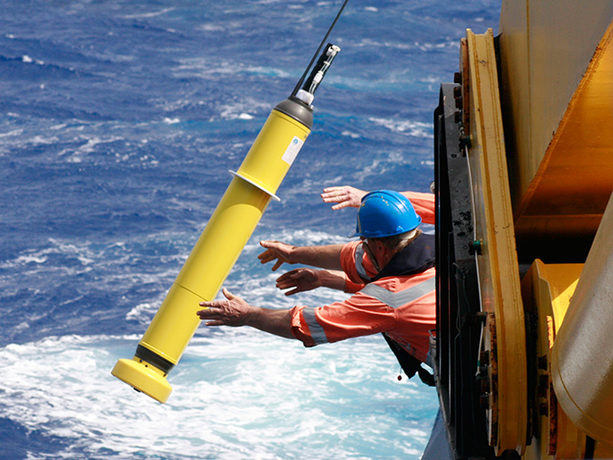
\includegraphics[width=.7\textwidth]{fig/L3/argo-float.jpg}\\
         \end{figure}
         \pause
              \column{.6\textwidth}
\begin{figure}
         \caption*{It measures several \textit{in-situ}  oceanic parameters}
         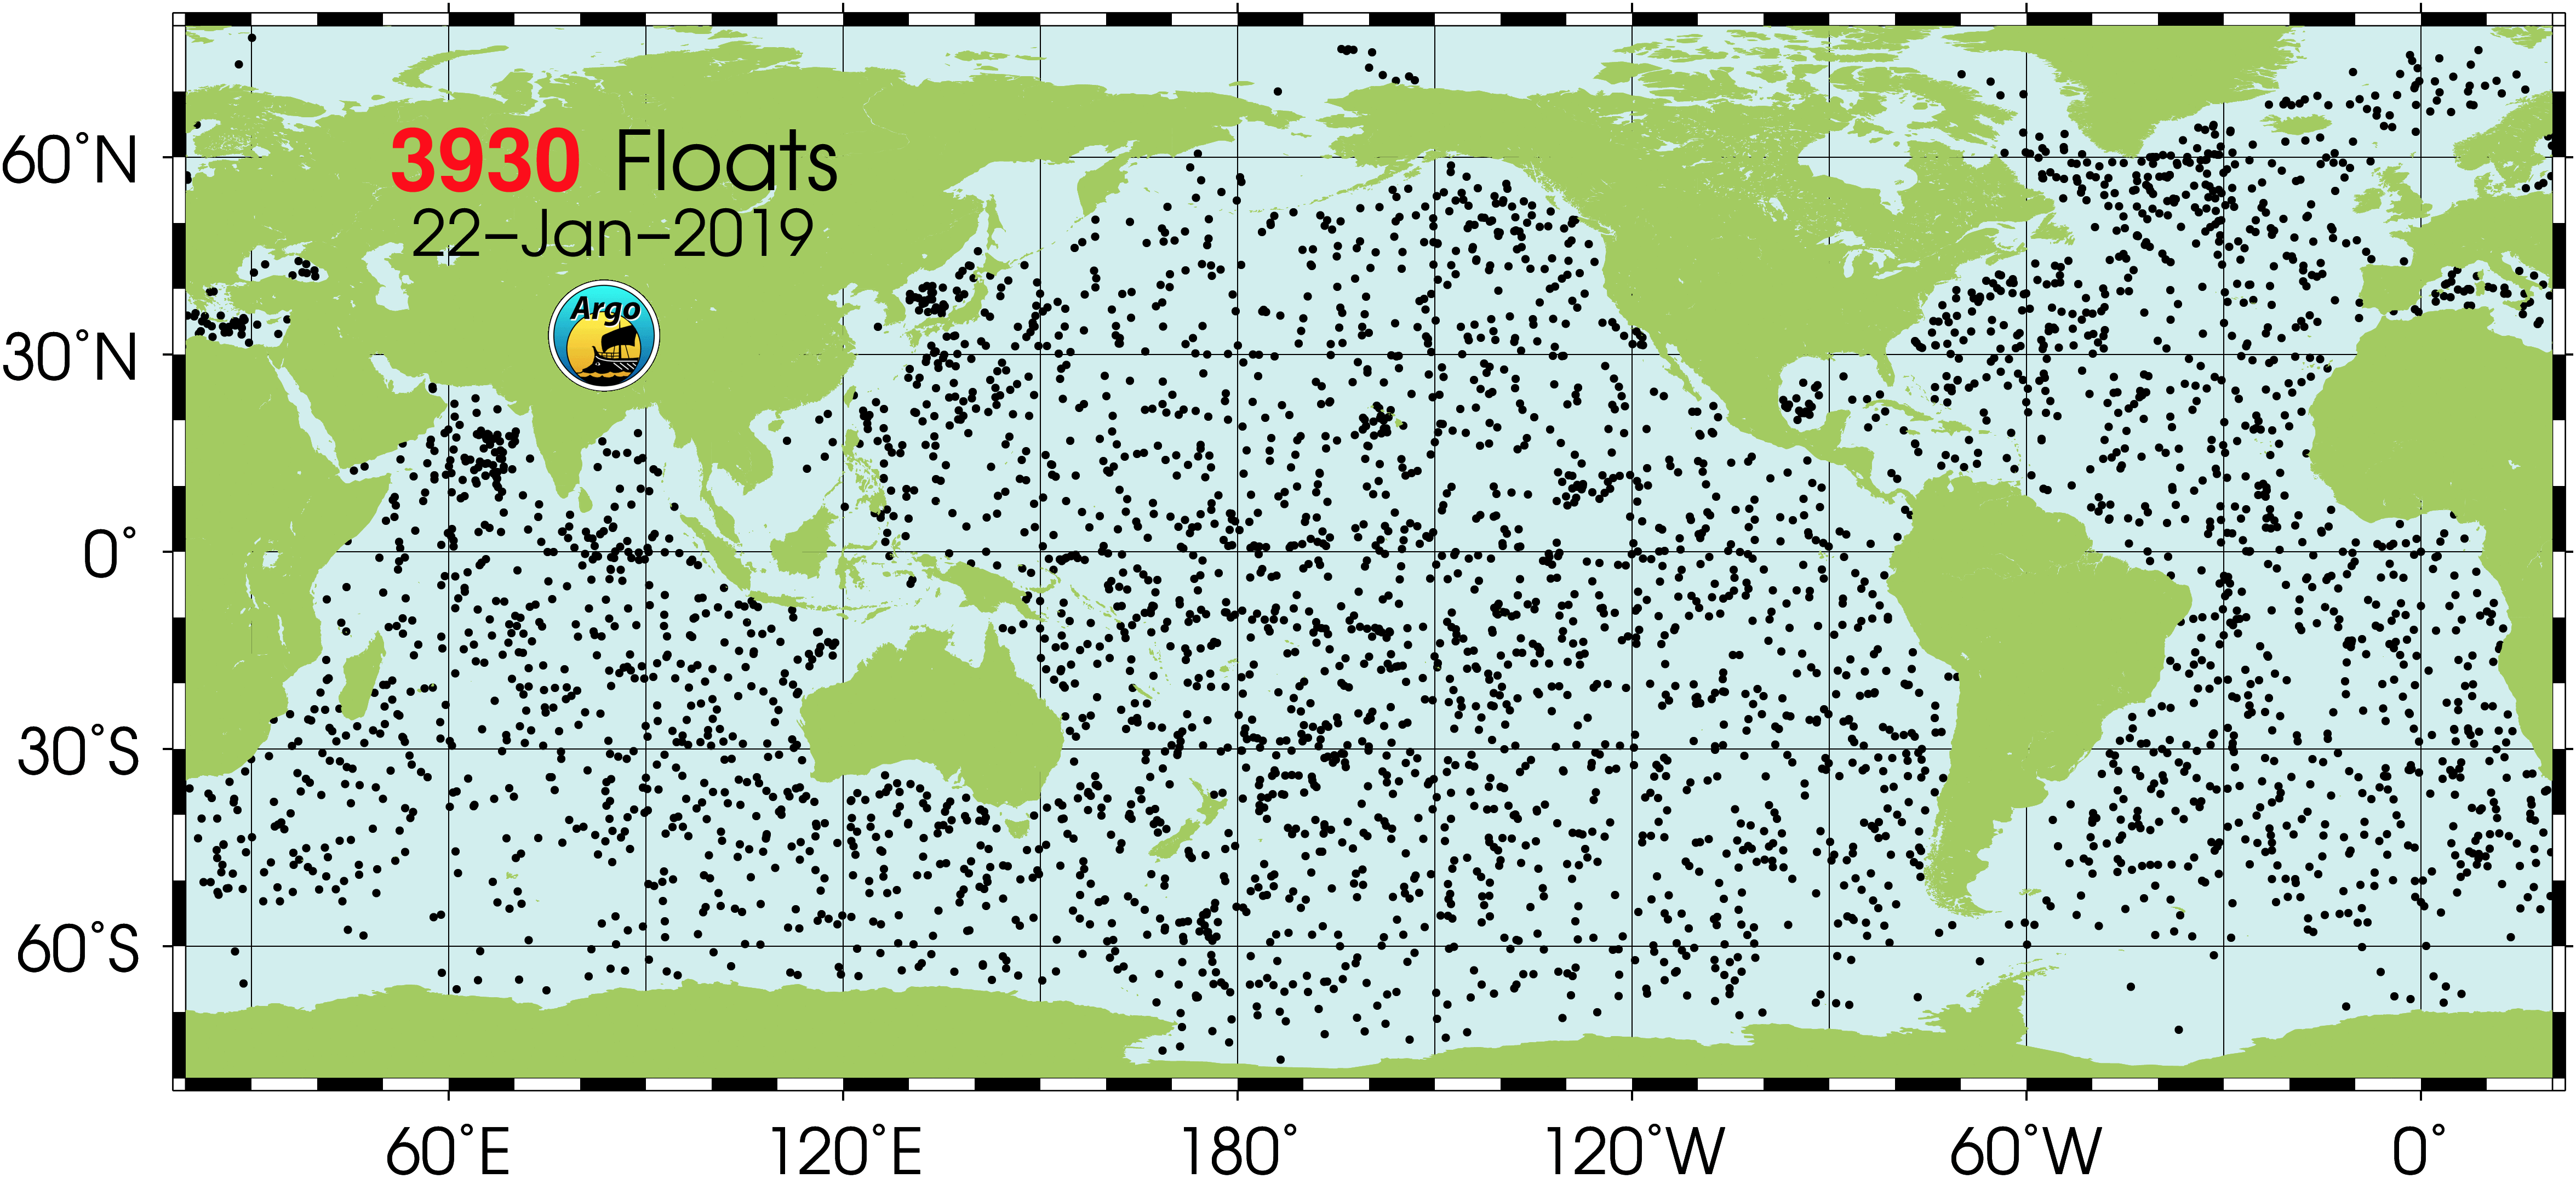
\includegraphics[width=\textwidth]{fig/L3/argo-status.png}
    \end{figure}

    \end{columns}
    
    \begin{columns}
   \pause
    \column{.6\textwidth}
    Matching between:
    \begin{itemize}
        \item Sparse \textit{in-situ} velocity at 1000m
        \item global surface velocity from satellite Sea-Surface heights (SSH).
    \end{itemize}
    \column{.4\textwidth} 
    \begin{figure}
         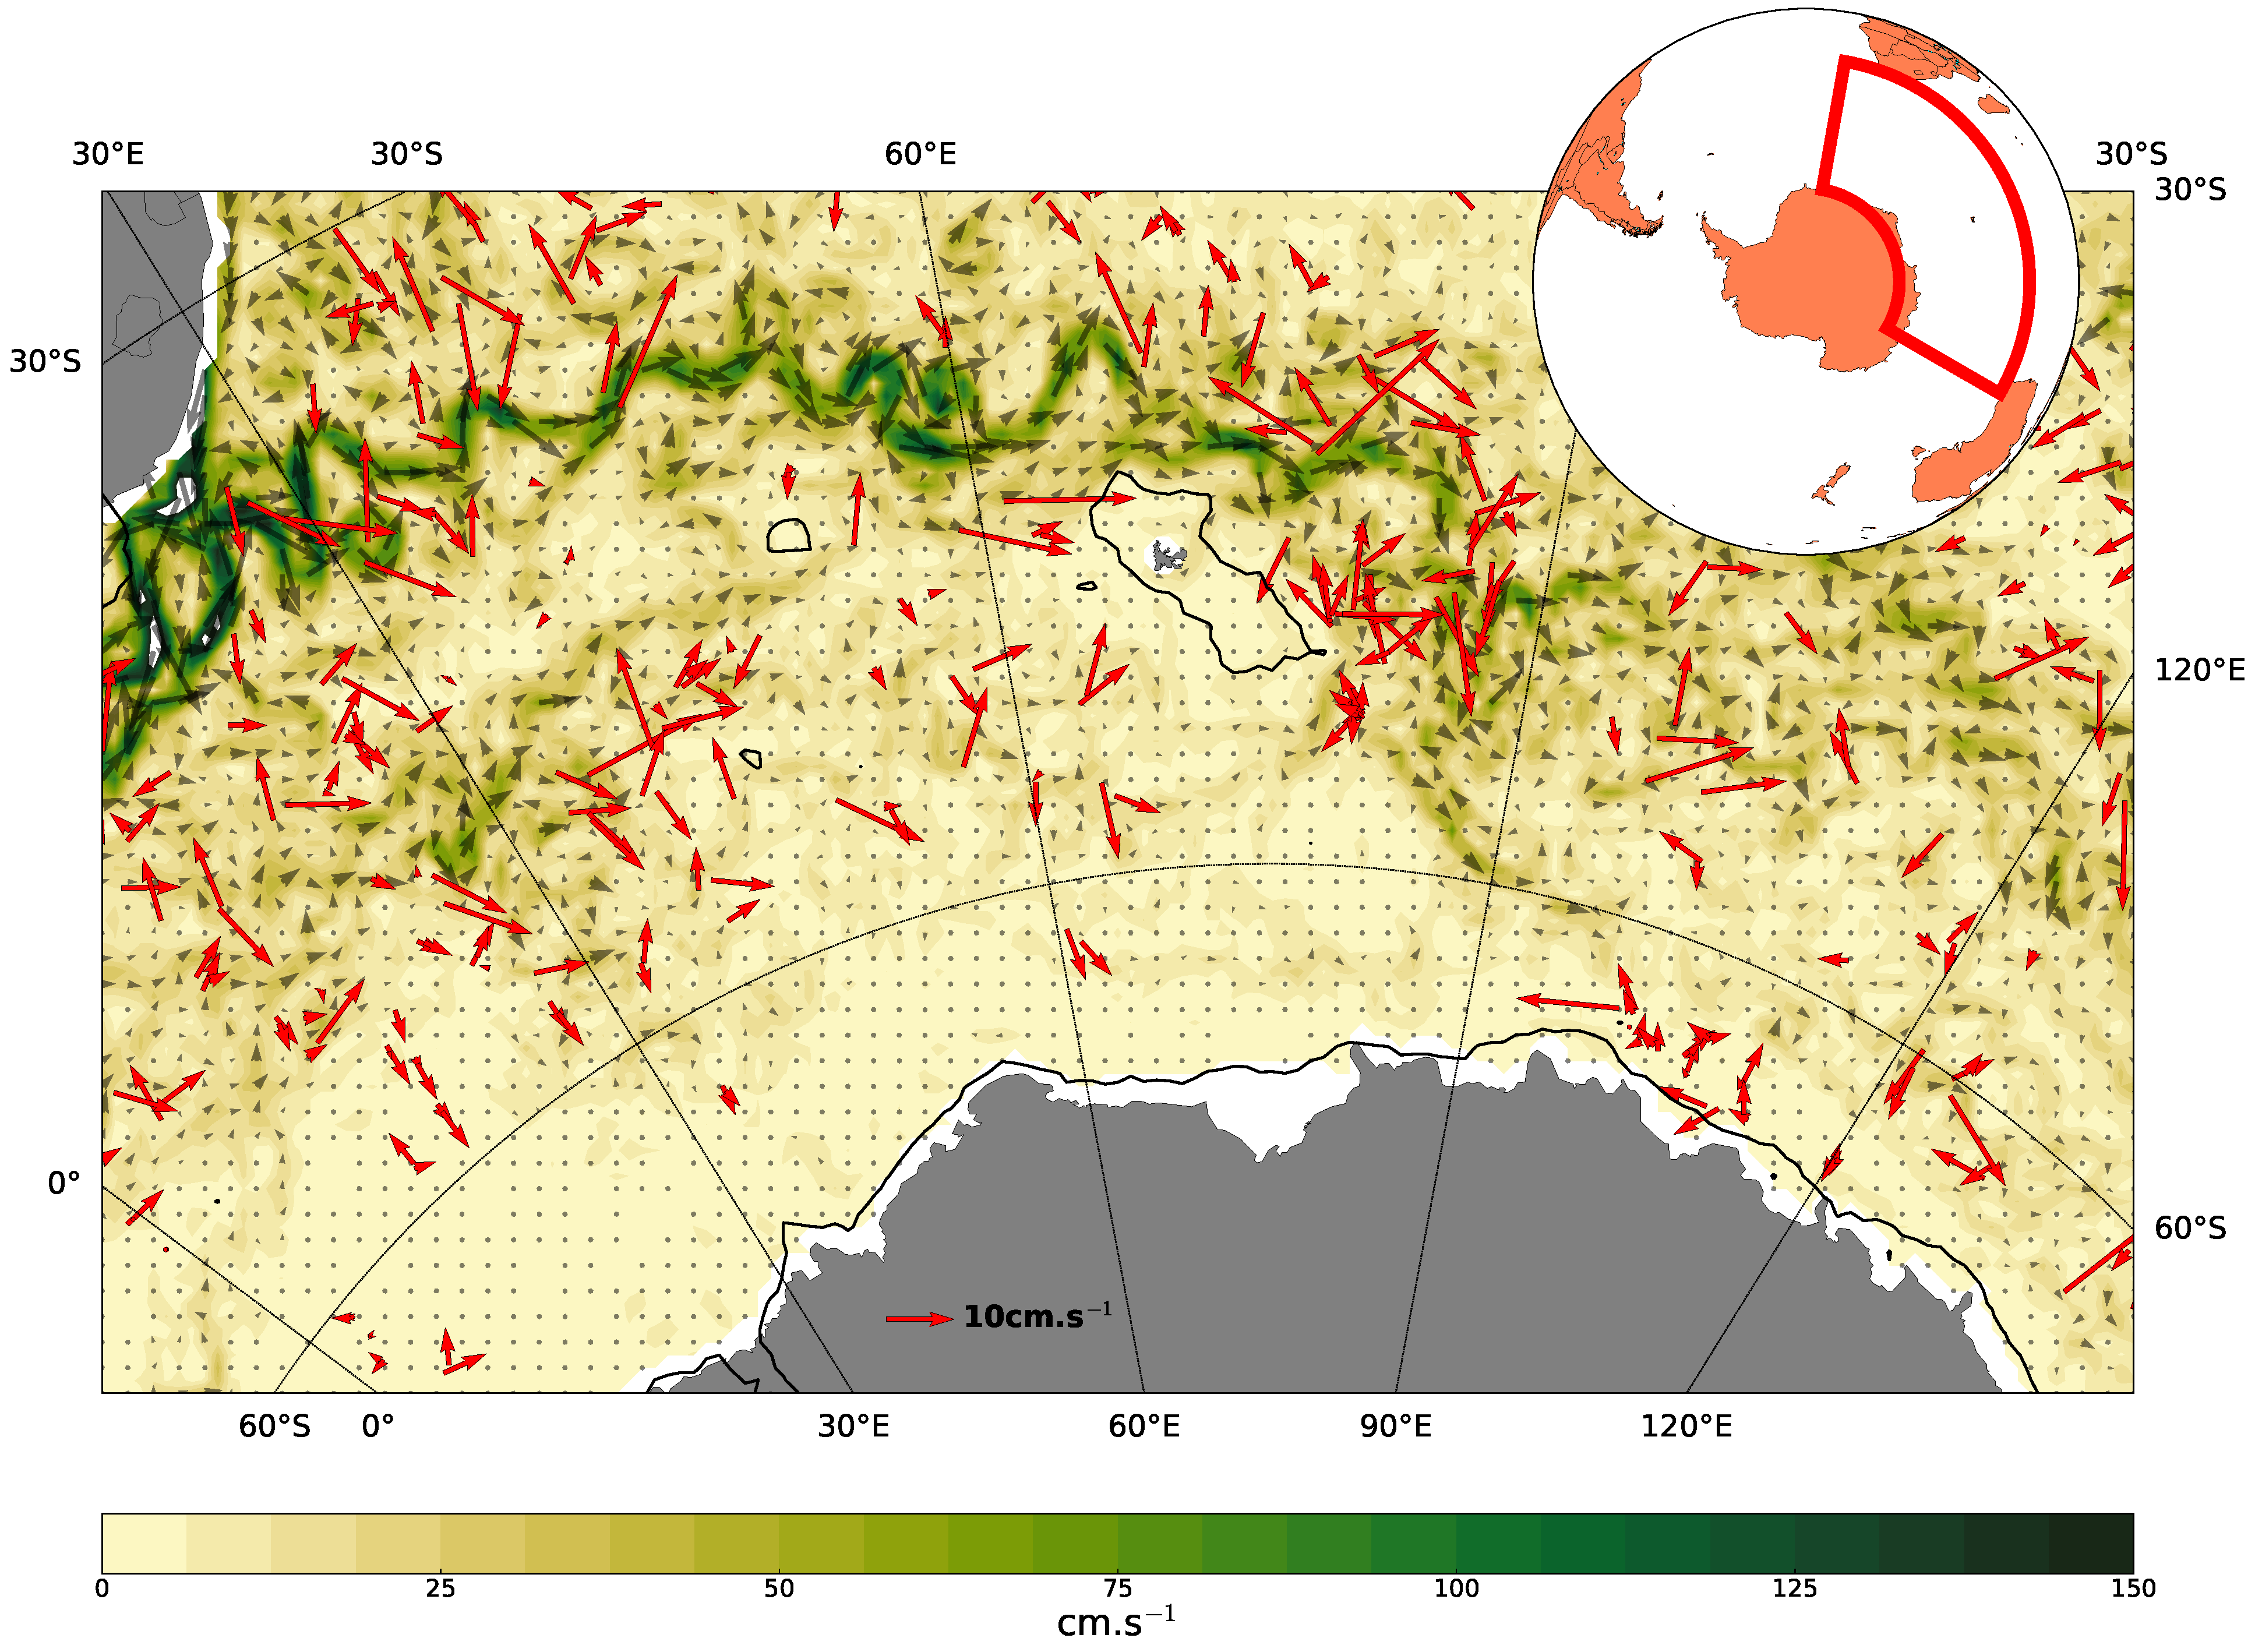
\includegraphics[width=\textwidth]{fig/L3/Surface_Currents_Kerguelen_Intro_resized_v2.pdf}
    \end{figure}
    
    \end{columns}
    \end{frame}
    
    \begin{frame}{Inference of unknown parameters}
        \begin{columns}
        \column{.6\textwidth}
                \rref[\cite{Chapman2017ReconstructionMaps}]

         \begin{figure}
         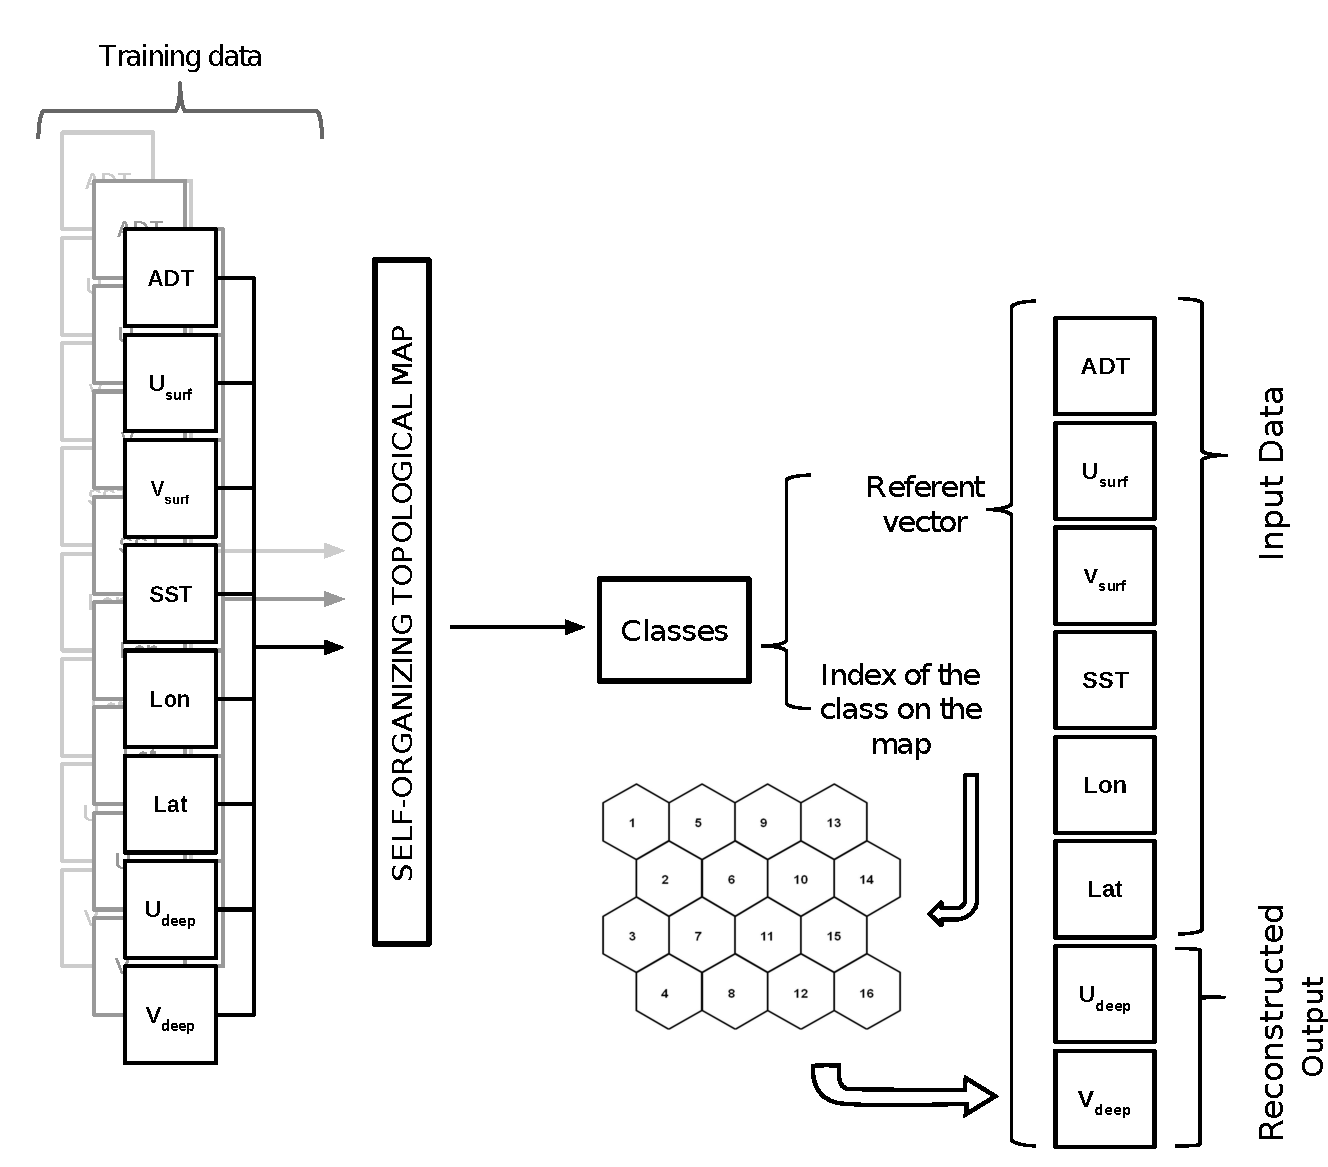
\includegraphics[width=\textwidth]{fig/L3/Method_Schematic_Modified.pdf}
    \end{figure}
    \pause
        \column{.4\textwidth}
         \begin{figure}
         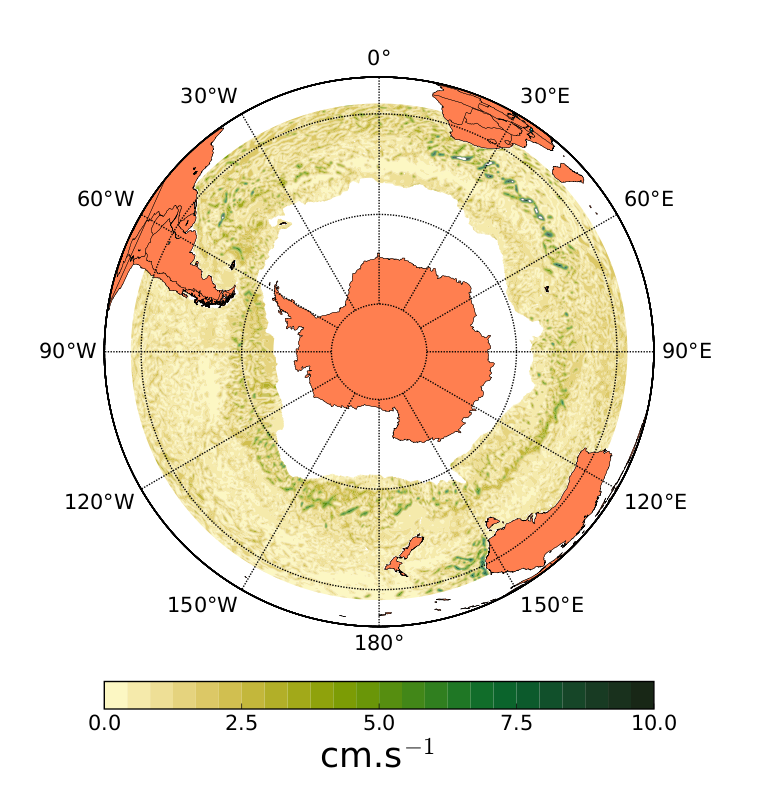
\includegraphics[width=\textwidth]{fig/L3/Deep_Mean_2009_Recon_resized_crop.png}\\
          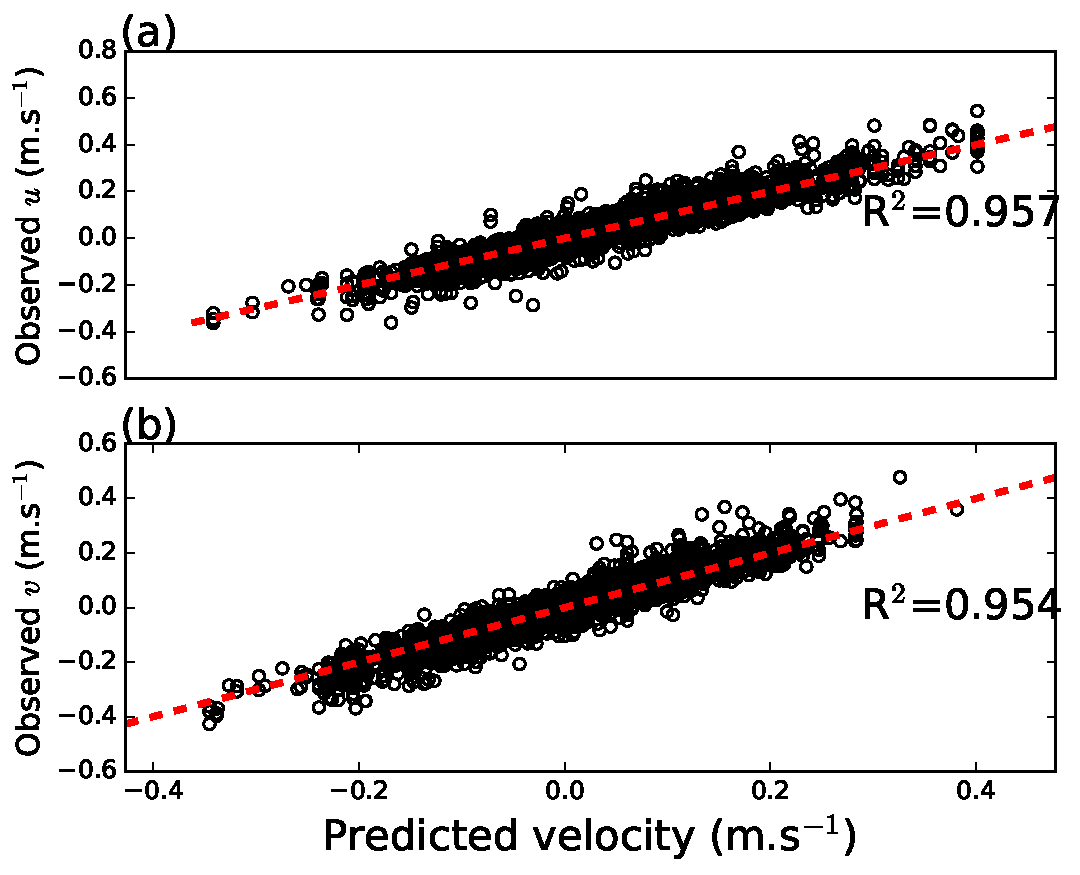
\includegraphics[width=\textwidth]{fig/L3/Scatter_uv_obs_vs_predict_resize.pdf}
    \end{figure}
        \end{columns}
    \end{frame}

\section{Machine learning and differential equations}
\begin{frame}{phyical system and differential equations}
    For example, Motion fluid can be represented using Navier-Stokes equations (PDE):
    
    $$ {\partial{\bf u}\over{\partial t}} = -  ({\bf u} \cdot \nabla) {\bf u} - {1\over\rho} \nabla p + \gamma\nabla^2{\bf u} + {1\over\rho}{\bf F} 
    $$
    \pause
    After spatial discretization, can be represented as an ODE:
    $$
    \frac{d\mathbf{x}}{dt} = f(\mathbf{x(t))}
    $$
\end{frame}

\begin{frame}{ResNET and ODE}
\begin{columns}
\column{.5\textwidth}
Euler discretization scheme:
$$
 x(t+\Delta t) = x + \Delta t.f(x(t)) 
$$
\pause
\column{.5\textwidth}
    \begin{figure}
    \centering
    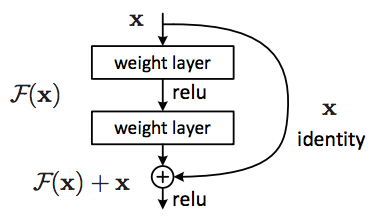
\includegraphics[width=.9\textwidth]{fig/L2/res_block.png}

    \end{figure}
    input: $x(t)$~\\ output:$x(t+\Delta t)$
    $$
    x(t+\Delta t) = x(t) + \Delta t.\mathcal{F}(x(t)) 
    $$
    
    \end{columns}
    \pause
    \alert{Training a ResNet is equivalent to training the underlying model in a Euler discretization scheme}
\end{frame}
\begin{frame}{Other schemes?}
\begin{columns}
\column{.5\textwidth}
\rref[\cite{Fablet2017}]

Runge-Kutta (order 4) integration scheme:
$$
x(t+\Delta t) = x(t) + \sum_{i=1}^4 \alpha_i k_i
$$
where $k_i = f(x(t+\beta_i k_{i-1}\Delta t))$\\
$k_0=0$, 
$\alpha_1=\alpha_4=1/6$,
$\alpha_2=\alpha_3=2/6$,
$\beta_1=\beta_4=1$ 
and  $\beta_2=\beta_3=1/2$.
\pause
\column{.5\textwidth}
\begin{figure}
    \centering
    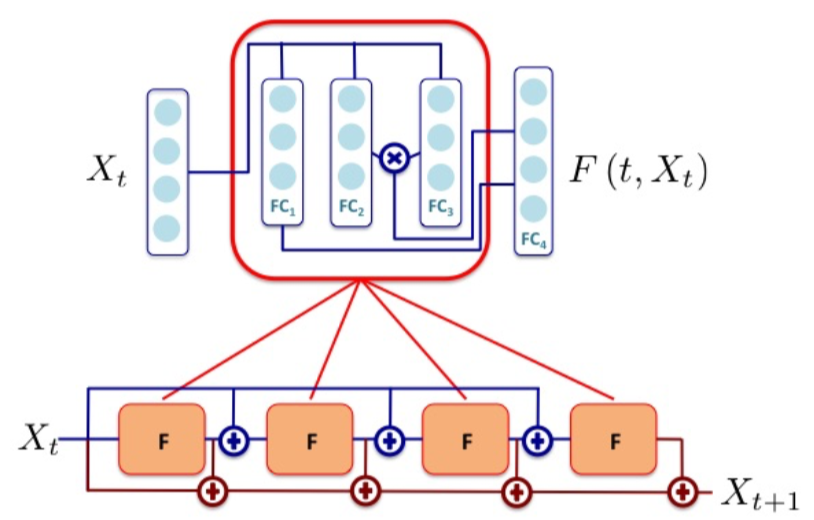
\includegraphics[width=\textwidth]{fig/L3/rk-resnet.png}\\
    \pause
      \caption*{Example on data simulated with a Lorenz 63 system}
     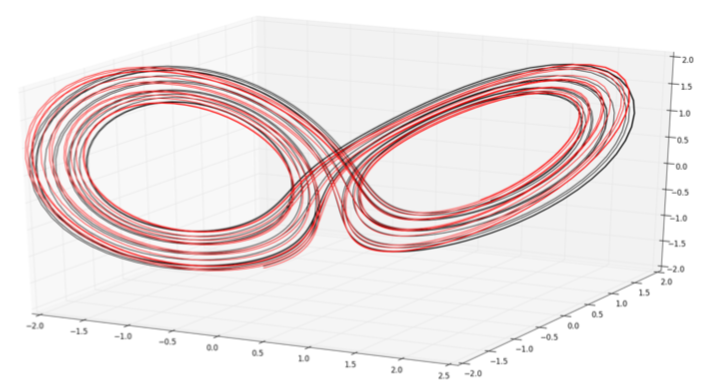
\includegraphics[width=\textwidth]{fig/L3/result-resnet.png}\\
   
\end{figure}
\end{columns}
\end{frame}

\begin{frame}{Toward general framework: Neural ODE}
    \rref[\cite{Chen2018NeuralEquations}: Best paper award NeurIPS, Dec. 2018]
    $$
    \mathbf{z}(t_1) = \mathbf{z}(t_0)  + \int_{t_0}^{t_1} f(\mathbf{z}(t),\theta) dt = \textrm{ODESolve}(\mathbf{z}(t_0),f,t_0,t_1,\theta)
    $$
    \begin{columns}
    \column{.5\textwidth}
    \begin{figure}
        \centering
        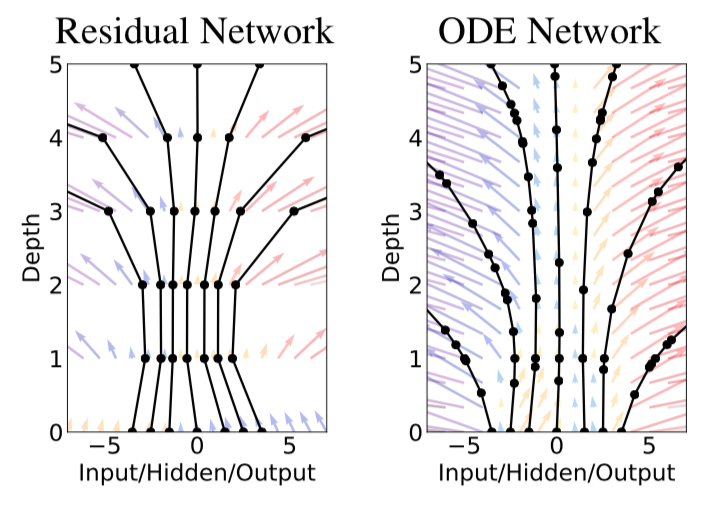
\includegraphics[width=\textwidth]{fig/L3/resVsODE.png}
    \end{figure}
    \column{.5\textwidth}
        \begin{figure}
        \centering
        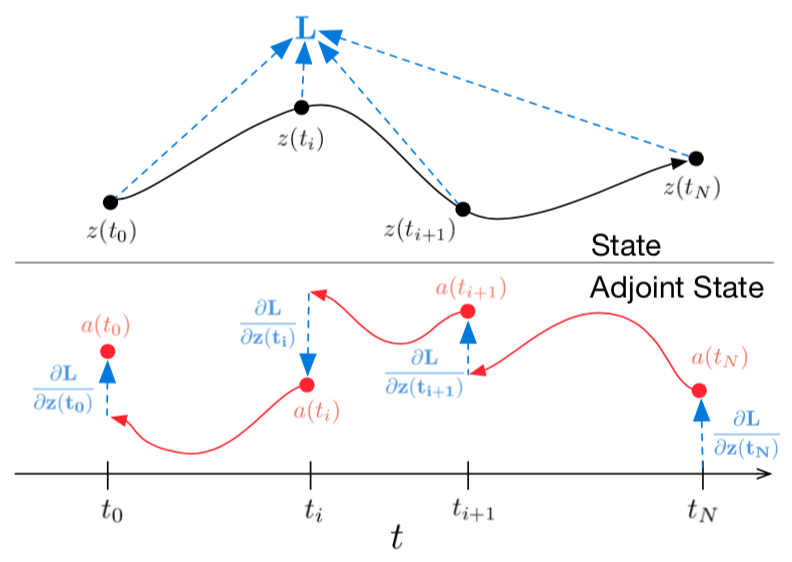
\includegraphics[width=\textwidth,trim={0 5.4cm 0 0},clip]{fig/L3/ODEscheme.png}
    \end{figure}
    \end{columns}
\end{frame}

\begin{frame}{Gradient backpropagation}
\begin{block}{Objective}
Computing $\partial L/ \partial \theta$
\end{block}
 \begin{columns}
   
    \column{.4\textwidth}
        \begin{figure}
        \centering
        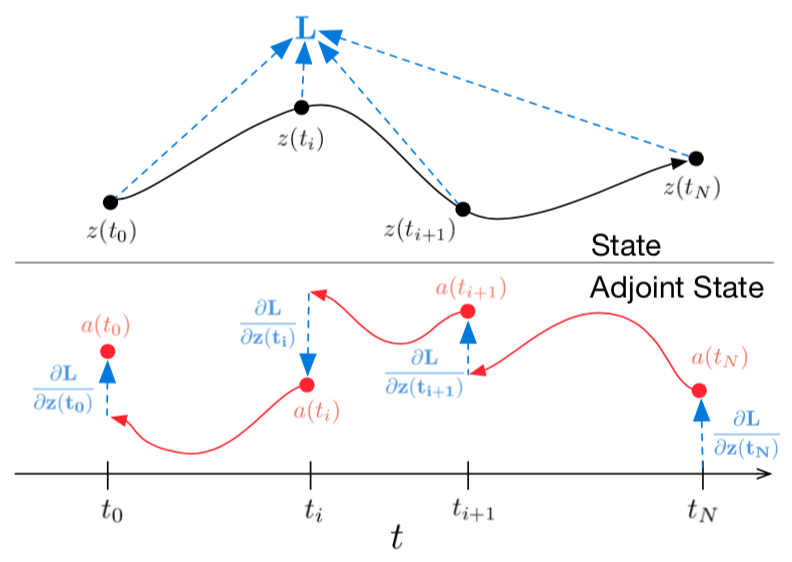
\includegraphics[width=\textwidth]{fig/L3/ODEscheme.png}
    \end{figure}
    \column{.6\textwidth}
    $\mathbf{z}(t_1) = \mathbf{z}(t_0)  + \int_{t_0}^{t_1} f(\mathbf{z}(t),\theta) dt$\\
    Define the adjoint:\\
    $\mathbf{a}(t)=\partial L / d\mathbf{z}(t)$\\
    $$\mathbf{a}(t_0)=\mathbf{a}(t_1) -\int_{t_1}^{t_0} a(t)^T \frac{\partial d f(\mathbf{z(t)},\theta)}{\partial \mathbf{z}}dt$$
      $$\frac{d L}{d\theta}=-\int_{t_1}^{t_0} a(t)^T \frac{\partial d f(\mathbf{z(t)},\theta)}{\partial \theta}dt$$
    
    $a(t)$ and $\frac{d L}{d\theta}=$ can be computed using the Same ODE solver backward in time.
    \end{columns}
\end{frame}

\section{Merge approaches: between physics and machine learning}
\begin{frame}
\frametitle{What is this about?}
\begin{tikzpicture}[%
  % common options for blocks:
  block/.style = {draw, fill=blue!30, align=center, anchor=west,
              minimum height=0.65cm, inner sep=0},
  % common options for the circles:
  ball/.style = {circle, draw, align=center, anchor=north, inner sep=0, text width=2cm,  minimum height=0.5cm},
  node distance=3.cm]]
  \node<1->[ball,fill=blue!30,] (pl) {Physical laws};
  \node<1->[ball,fill=blue!30, right of=pl] (nm) {Numerical models};
   \node<2->[ball,fill=red!30, right of=nm] (ml) {Machine Learning};
  \node<2->[ball,fill=red!30, right of=ml] (d) {Data};
  \draw<1->[->,very thick,draw=blue!50] (pl.east) -- (nm.west);
  \draw<2->[->,very thick,draw=red!50] (d.west) -- (ml.east);
  \draw<3->[<->,very thick] (nm.east) -- (ml.west) node[midway, above]{?} ;
  \end{tikzpicture}
\end{frame}

\begin{frame}{SST dynamic}
    \rref[\cite{DeBezenac2017TowardsModeling}]
    \begin{block}{Objective}
    Given $SST(t-h),\cdots,SST(t)$, predict $SST(t+\tau)$
    \end{block}
    \begin{columns}
    \column{.5\textwidth}
    \begin{figure}
        \centering
        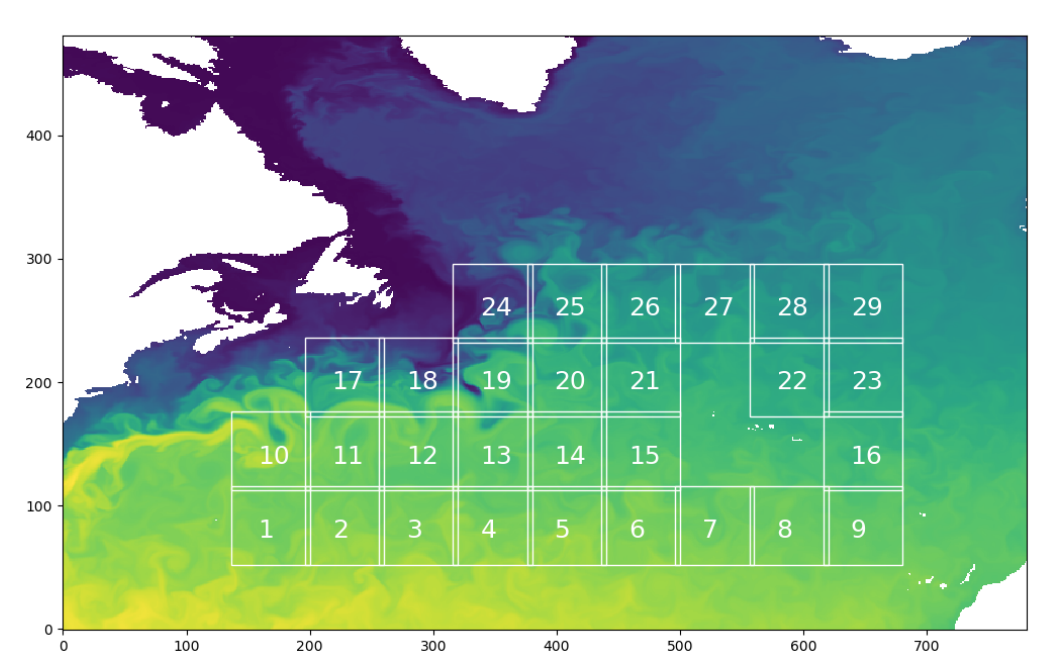
\includegraphics[width=\textwidth]{fig/L3/sst-map.png}
    \end{figure}
    \pause
    \column{.5\textwidth}
   \begin{figure}
        \centering
        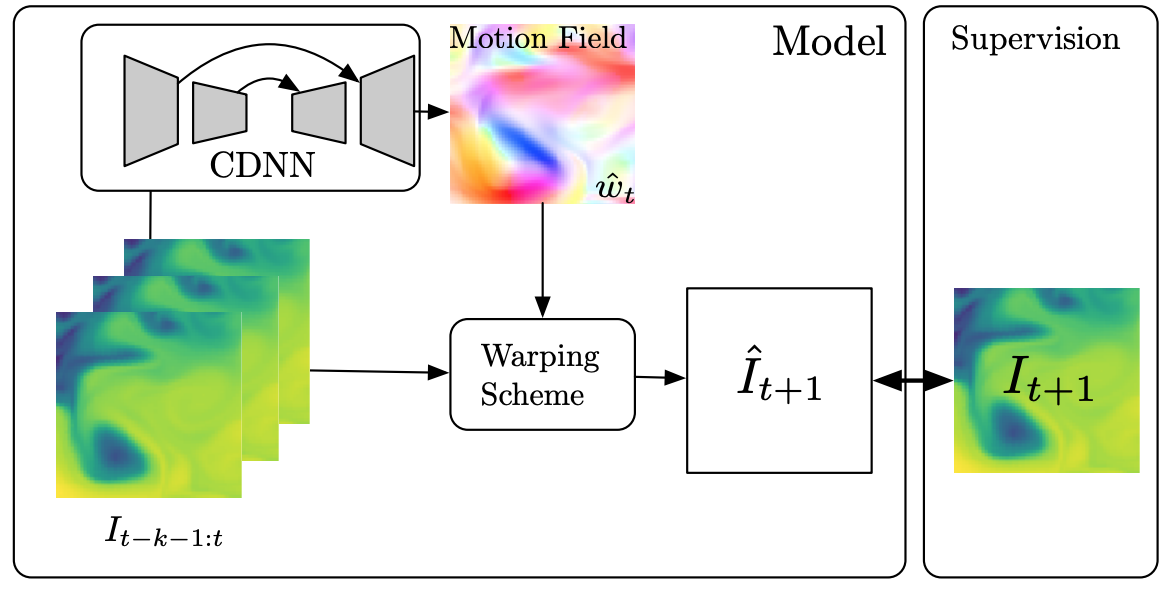
\includegraphics[width=\textwidth]{fig/L3/sst-nn-scheme.png}
    \end{figure}
        \end{columns}

\end{frame}

\begin{frame}{Illustration}
\begin{figure}
\begin{tikzpicture}
\begin{scope}[text width=8em,anchor=east, align=right]
\node (line2) {Deep learning forecast};
\node [above of = line2,node distance = 1.2cm] (line1) {Reanalysis (truth)};
\node [below of = line2,node distance = 2cm] (line3) {Motion estimate};
\end{scope}
\node [right of = line2, anchor=west, node distance = 1.8cm] (im) {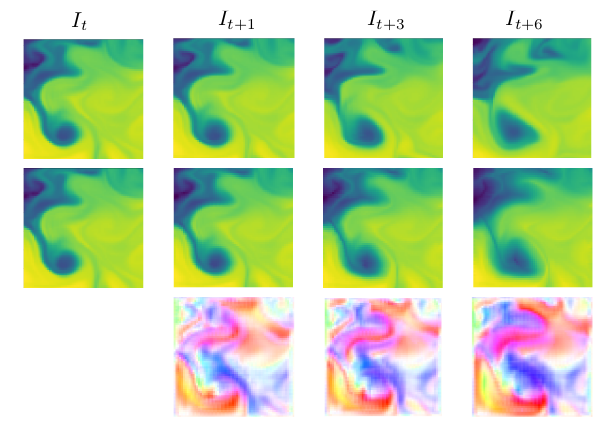
\includegraphics[height=5cm]{fig/L3/sst-predict.png}};
\end{tikzpicture}
\end{figure}
\end{frame}
%%%%%%%%%%%%%%%%%%%%
\begin{frame}
\frametitle{Other problem}
Using a numerical model $\M$, we can simulate
 the evolution in time of a state vector $\x(t)$:

\begin{equation*}
\frac{d\x}{dt} = \M_0(\x(t))
\end{equation*}
Some processes cannot be exactly resolved using only physical
principles, because of:
\begin{itemize}
\item Imperfect physical knowledge
\item Numerical schemes
\item Discretization errors
\item Unknown factors
\end{itemize}
In practice, the unresolved/unknown processes can be represented by a 
%JS j'ai remplace an par a 
$\btheta$:
\begin{equation*}
\frac{d\x}{dt} = \M(\x(t),\btheta)
\end{equation*}
\end{frame}
%%%%%%%%%%%%%%%%%%%%
\begin{frame}
\frametitle{Determination of $\btheta$}
\begin{equation*}
\frac{d\x}{dt} = \M(\x(t),\btheta(t))
\end{equation*}
    $\theta$ must be determined to produce a fair simulation.
\pause[2]
\alert{Method:}    $\btheta$ is determined using a data-driven approach.\\
\vspace{1em}
\pause[3]
Two approaches:
\begin{itemize}
\item <3-> {\color<5>{gray}$\theta$ is estimated directly by fitting some observations (Data assimilation)}
\item <4->\alert<5>{ $\theta$ is calculated by using an empirical model $f$  :
%JS j'ai ajoute using; ajouter numerical apres empirical ?
\begin{equation*}
\btheta(t) = f(\x(t))
\end{equation*}}
\end{itemize}
\pause[5]
\begin{alertblock}{Question:}
Can $f(\x(t))$ be represented by a neural network ?
\end{alertblock}
\end{frame}

%%%%%%%%%%%%%%%%%%%%%
\begin{frame}
\frametitle{Proof of concept using a shallow-water model}
%As a proof of concept, we used a shallow-water model:
\vspace{-1.5em}
\begin{eqnarray}
\partial_tu & = &
+ (f + \zeta ).v  - \partial_x (\frac{u^2+v^2}{2} + g^*.h) + \textcolor{red}{\btheta_u}\nonumber \\
\partial_tv & = &
-  (f + \zeta ).u  - \partial_y (\frac{u^2+v^2}{2} + g^*.h) + \textcolor{red}{\btheta_v}\nonumber \\
\partial_th & = &
- \partial_x(u(H+h)) - \partial_y(v(H+h)) \nonumber
\end{eqnarray}

%\footnotesize
\vspace{.5em}
\pause
\begin{block}{Validation of the approach}
To validate our approach, we use reference synthetic data produced by a
fully-specified shallow-water model :
\begin{eqnarray*}
\btheta_u& =  f_u(u,h,\tau_x)  = & \frac{\tau_x}{\rho_0(H+h)} - \gamma . u + \nu\Delta u\\
\btheta_v &=  f_v(v,h,\tau_y)  = & \frac{\tau_y}{\rho_0(H+h)} - \gamma . v + \nu\Delta v 
\end{eqnarray*}
\end{block}
\end{frame}


%%%%%%%%%%%%%%%%%%%%
\begin{frame}
\frametitle{Diagnostic quantities of the reference simulation}
\framesubtitle{15 years of simulation after a 10 years spinup}
\begin{columns}
\column{.4\textwidth}
\centering
{\footnotesize mean $h$ }\\
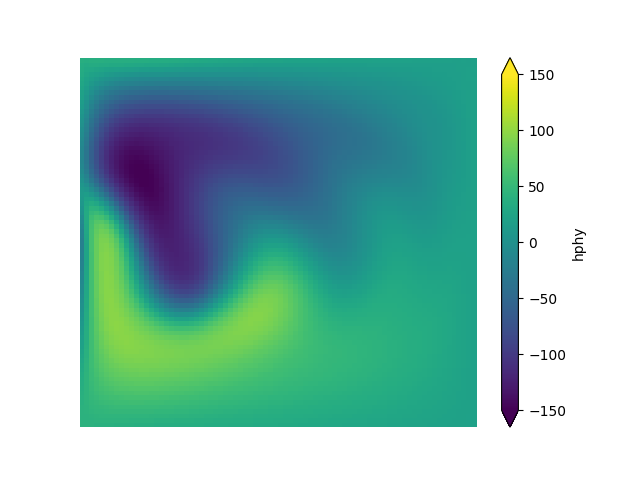
\includegraphics[width=\textwidth]{./fig/L3/mean-hphy0.png}\\
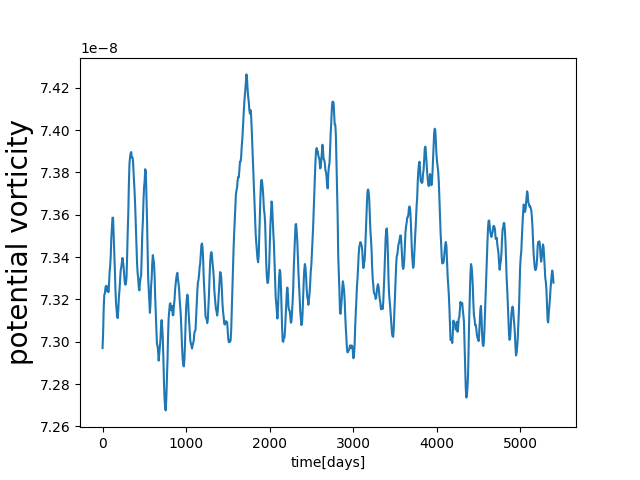
\includegraphics[width=\textwidth]{./fig/L3/evol-0--PV.png}

\column{.4\textwidth}
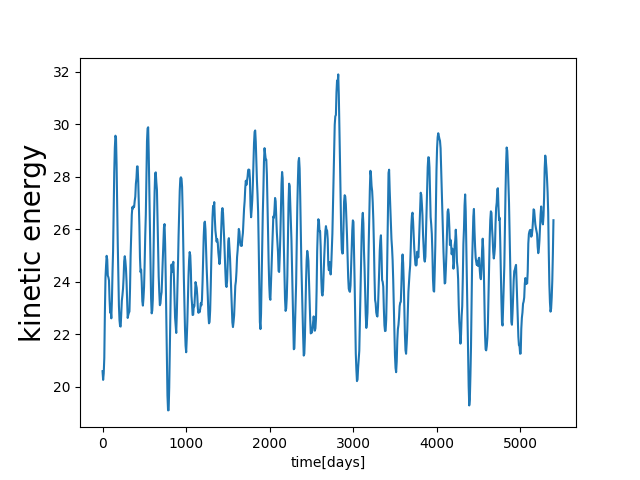
\includegraphics[width=\textwidth]{./fig/L3/evol-0--EC.png}\\
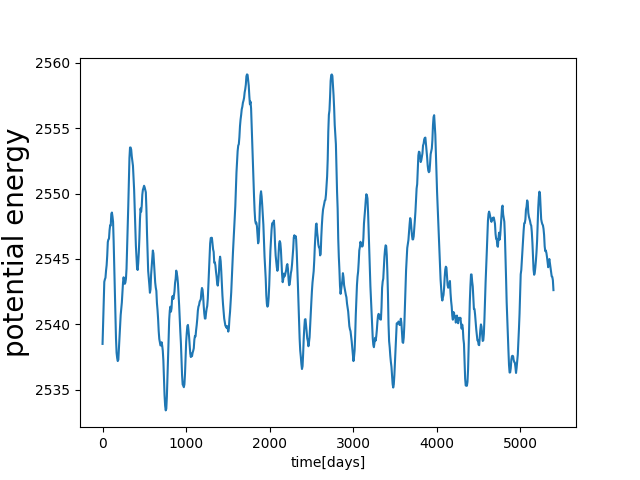
\includegraphics[width=\textwidth]{./fig/L3/evol-0--EP.png}
\end{columns}


\end{frame}


%%%%%%%%%%%%%%%%%%%%
\begin{frame}
\frametitle{Training dataset}
After a simulation of the reference model 
$\M_T$, we have a set of $\sim 300$ examples of mapping between 
$\x = (u,v,h)$ and $\btheta$ :

\begin{table}
\begin{tabular}{|ccc|c|}
\hline
\multicolumn{3}{|c|}{Input} & Output \\
\hline
$u$ &  $h$ & $\tau_x$ & $\theta_u $ \\
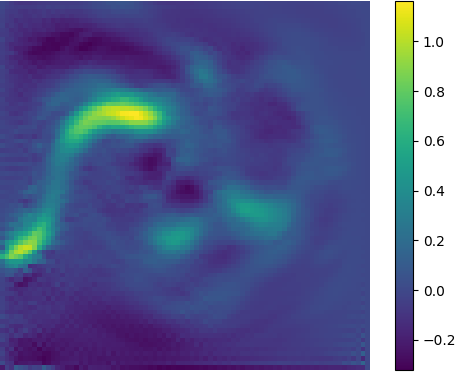
\includegraphics[width=.22\textwidth]{./fig/L3/trainset-u.png} &
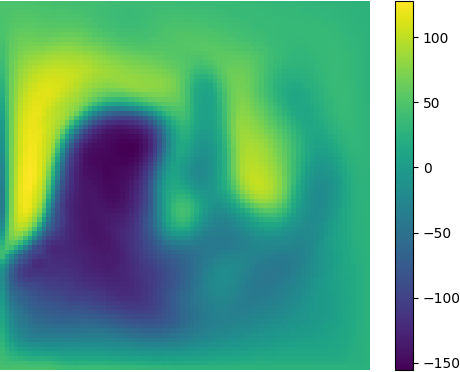
\includegraphics[width=.22\textwidth]{./fig/L3/trainset-h.png} &
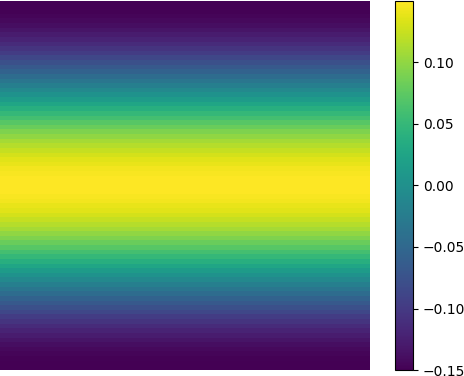
\includegraphics[width=.22\textwidth]{./fig/L3/trainset-tau.png} &
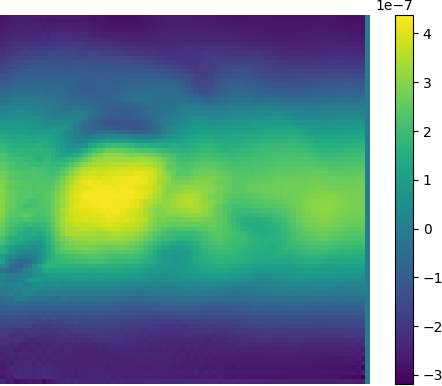
\includegraphics[width=.22\textwidth]{./fig/L3/trainset-uparam.png}\\
\hline
$v$ &  $h$ & $\tau_y$ & $\theta_v $ \\
\hline
\end{tabular}
\end{table}


\end{frame}

%%%%%%%%%%%%%%%%%%%%%%
\begin{frame}
\frametitle{Description of the neural networks}
\def\layersep{2.5cm}
\begin{tikzpicture}[shorten >=1pt,->,draw=black!50, node distance=\layersep]
    \tikzstyle{every pin edge}=[<-,shorten <=1pt]
    \tikzstyle{neuron}=[circle,fill=black!25,minimum size=17pt,inner sep=0pt]
    \tikzstyle{input neuron}=[draw=black,minimum size=17pt,inner sep=2pt];
    \tikzstyle{output neuron}=[neuron, fill=red!50];
    \tikzstyle{hidden neuron}=[neuron, fill=blue!50];
    \tikzstyle{missing neuron}=[]
    \tikzstyle{annot} = [text width=5em, text centered]

    % Draw the input layer nodes
    \node[input neuron, pin=left:$u$] (I-1) at(0,-1.5)
    {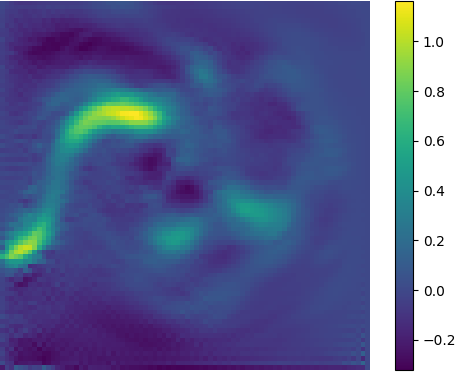
\includegraphics[width=.1\textwidth]{./fig/L3/trainset-u.png}};
    
    \node[input neuron, pin=left:$h$] (I-2) at(0,-3)
    {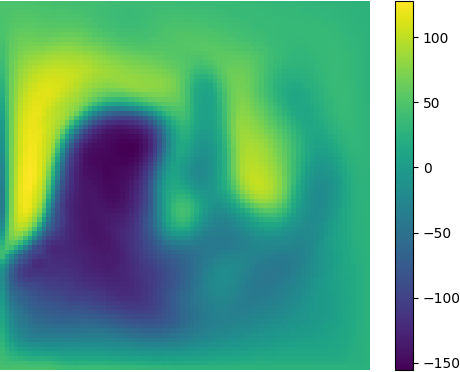
\includegraphics[width=.1\textwidth]{./fig/L3/trainset-h.png}};
    
    \node[input neuron, pin=left:$\tau_x$] (I-3) at(0,-4.5)
    {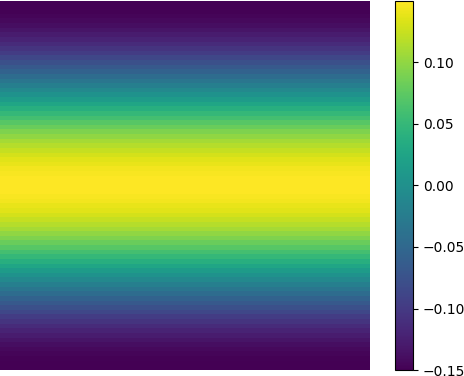
\includegraphics[width=.1\textwidth]{./fig/L3/trainset-tau.png}};
    
    % Draw the first hidden layer
    \node[hidden neuron] (H-1) at (\layersep,-1) {};
    \node[hidden neuron] (H-2) at (\layersep,-2) {};
    \node[] (H-3) at (\layersep,-3) {$\vdots$};
    \node[hidden neuron] (H-4) at (\layersep,-4) {};
    \node[hidden neuron] (H-5) at (\layersep,-5) {};
    
    % Draw the second hidden layer
        
    \node[hidden neuron] (HH-1) at (2*\layersep,-1) {};
    \node[hidden neuron] (HH-2) at (2*\layersep,-2) {};
    \node[] (HH-3) at (2*\layersep,-3) {$\vdots$};
    \node[hidden neuron] (HH-4) at (2*\layersep,-4) {};
    \node[hidden neuron] (HH-5) at (2*\layersep,-5) {};
   
   	% Draw the output layer
    \node[input neuron, pin={[pin edge={->}]right:$\theta_u$}] (O) at (3*\layersep,-3) 
    {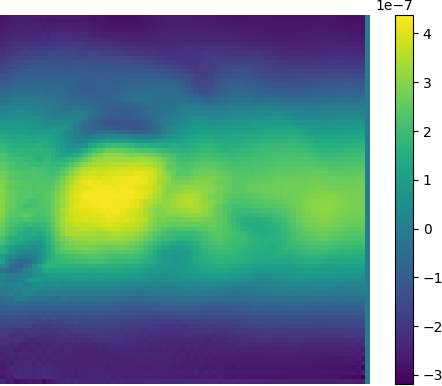
\includegraphics[width=.1\textwidth]{./fig/L3/trainset-uparam.png}};
   
   % Draw connections
   \foreach \source in {1,...,3}
        \foreach \dest in {1,2,4,5}
            \path (I-\source) edge (H-\dest);
    \foreach \source in {1,2,4,5}
        \foreach \dest in {1,2,4,5}
            \path (H-\source) edge (HH-\dest);
	\foreach \source in {1,2,4,5}
    		\path (HH-\source) edge (O) ;
    % Annotate the layers
  \node[annot,above of=H-1, node distance=1cm] (hl) {{\footnotesize
      Conv. layer\\ $3\times3$\\32 filters}};
    \node[annot,above of=HH-1, node distance=1cm] (hhl)
    {{\footnotesize Conv. layer\\ $1\times1$\\16 filters}};
    \node[annot,left of=hl] {Input layer};
    \node[annot,right of=hhl] {Output layer};
\end{tikzpicture}
Number of weights to optimize in the neural network : $\sim 1700$
\end{frame}

\begin{frame}
\frametitle{Spinup/Training/Validation}
\centering
\begin{tikzpicture}[%
]
%\filldraw[color=lightgray] (0,0) rectangle (2,2) node[pos=.5] {Test};        
\node[draw, fill=gray!20, fit={(0,0) (3,1.5)}, inner sep=0pt, label=center:Spinup] (A) {};
\node[draw, fill=blue!20, fit={(3,0) (8,1.5)}, inner sep=0pt, label=center:Training] (B) {};
\node[draw, fill=red!20, fit={(8,0) (11,1.5)}, inner sep=0pt, label=center:Test] (B) {};
%\draw [->,thick] (0,-0.5) -- (11.2,-0.5);
\draw [|-|,thick] (0,-0.5) -- (3, -.5) node[midway, below]{10 years};
\draw [-|,thick] (3,-0.5) -- (8, -.5) node[midway, below]{15 years};
\draw [->,thick] (8,-0.5) -- (11.1, -.5) node[midway, below]{10 years};
\end{tikzpicture}
\end{frame}

%%%%%%%%%%%%%%%%%%%%%%
\begin{frame}
\frametitle{Performance of the neural net}
\begin{columns}[t]
\column{.05\textwidth}
\begin{turn}{90}
Neural Netwotk output
\end{turn}
\column{.44\textwidth}
\centering
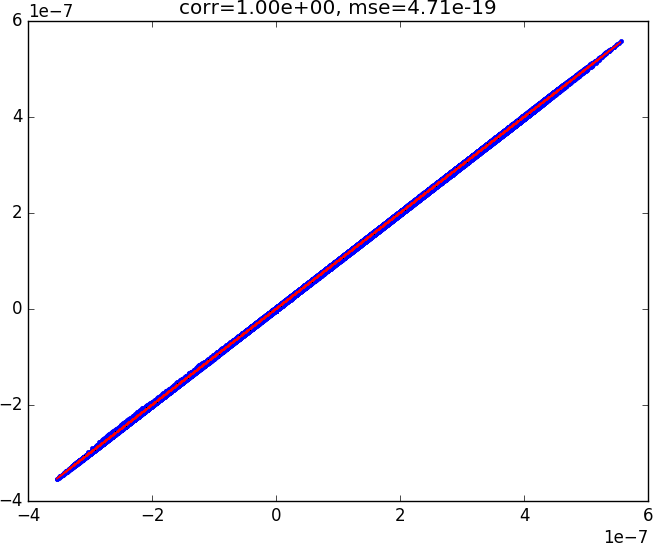
\includegraphics[width=\textwidth]{./fig/L3/scat_upar.png}\\
True $\theta_u$

\column{.44\textwidth}
\centering
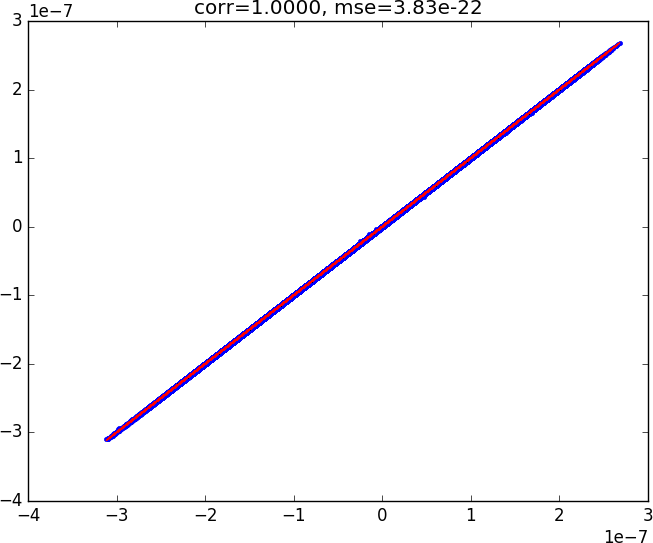
\includegraphics[width=\textwidth]{./fig/L3/scat_vpar.png}\\
True $\theta_v$
\end{columns}
\end{frame}

%%%%%%%%%%%%%%%%%%%%%%
\begin{frame}
\frametitle{Description of the neural net simulation}
Neural nets 
%$\theta_u = f_u(u,h,\tau_x)$ and $\theta_v = f_u(v,h,\tau_y)$ 
are inserted into the shallow-water model: 
\begin{eqnarray}
\partial_tu & = &
+ (f + \zeta ).v  - \partial_x (\frac{u^2+v^2}{2} + g^*.h) + \textcolor{red}{f_u(h,u,\tau_x)}\nonumber \\
\partial_tv & = &
-  (f + \zeta ).u  - \partial_y (\frac{u^2+v^2}{2} + g^*.h) + \textcolor{red}{f_v(h,v,\tau_y)}\nonumber \\
\partial_th & = &
- \partial_x(u(H+h)) - \partial_y(v(H+h)) \nonumber
\end{eqnarray}

$\textcolor{red}{f_u(h,u,\tau_x)}$ and $\textcolor{red}{f_v(h,v,\tau_y)}$ are the neural nets used to estimate $\btheta_u$ and $\btheta_v$
at each time step.
\end{frame}
%%%%%%%%%%%%%%%%%%%%%%
\begin{frame}
\frametitle{A first simulation}
\begin{columns}
\column{.3\textwidth}
\centering
{\footnotesize mean $h$ for true model}\\
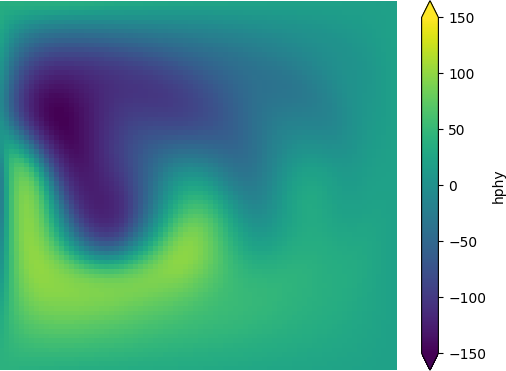
\includegraphics[width=\textwidth]{./fig/L3/meannw-hphy0.png}
\column{.3\textwidth}
\centering
{\footnotesize mean $h$ for nn model}\\
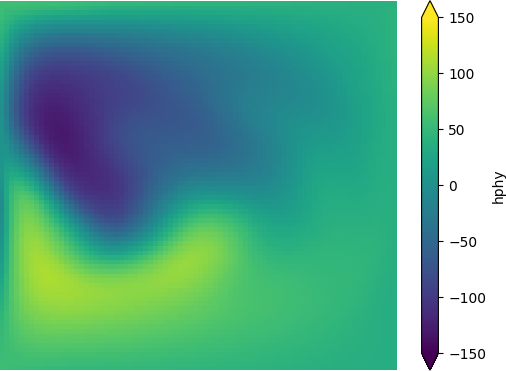
\includegraphics[width=\textwidth]{./fig/L3/meannw-hphy1.png}
\column{.3\textwidth}
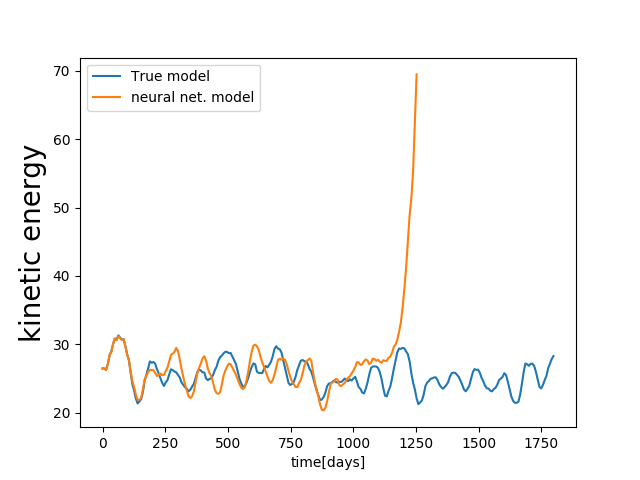
\includegraphics[width=\textwidth]{./fig/L3/evolnw-EC.png}\\
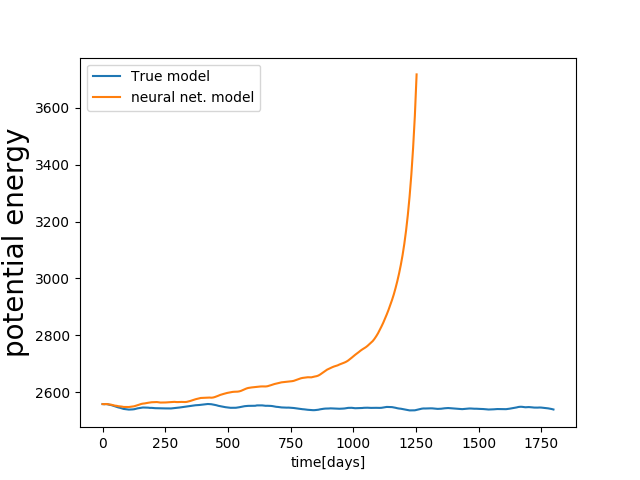
\includegraphics[width=\textwidth]{./fig/L3/evolnw-EP.png}
\end{columns}
\end{frame}

%%%%%%%%%%%%%%%%%%%%%
\begin{frame}
\frametitle{Are the boundary conditions was correctly represented ?}
\begin{columns}
\column{.5\textwidth}
Has the neural net learned $u=0$ velocity at the East boundary ?
\begin{figure}
\centering
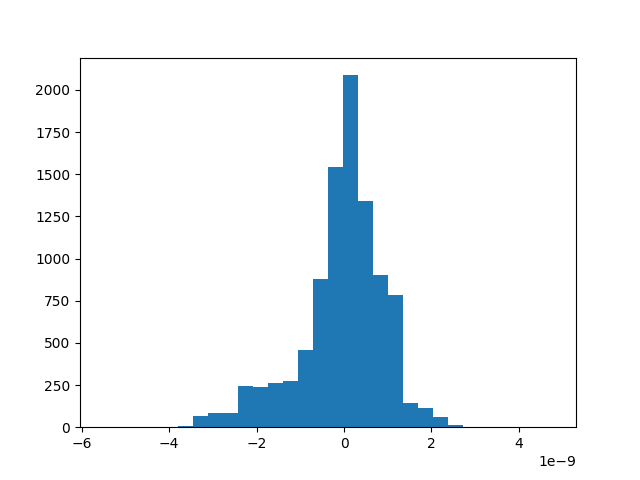
\includegraphics[width=\textwidth]{./fig/L3/u_veloocity_east.png}\\
histogram of $u$ values near the Eastearn boundary (RMS = $9.9e-10$)
\end{figure}
\pause
\column{.5\textwidth}
\begin{itemize}
\item Consequence : The NN model is not conservative : 
\begin{figure}
\centering
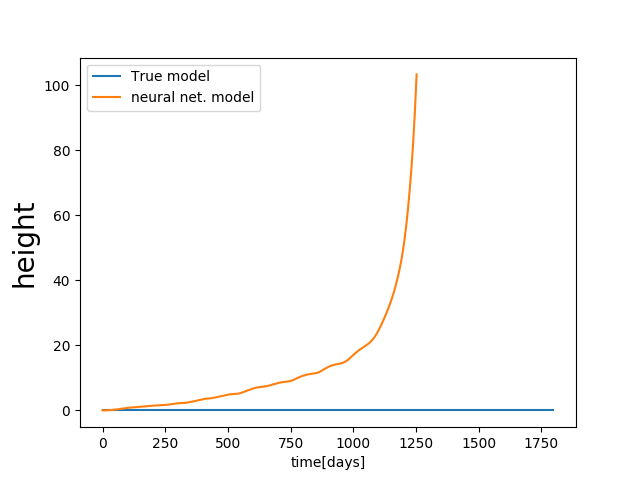
\includegraphics[width=\textwidth]{./fig/L3/evolnw-h}\\
Evolution of mean depth
\end{figure}
\item The boundary conditions have to be imposed.
\end{itemize}
\end{columns}
\end{frame}


%%%%%%%%%%%%%%%%%%%%%%
\begin{frame}
\frametitle{Simulation with imposed boundary conditions}
\begin{columns}

\column{.3\textwidth}
\centering
{\footnotesize mean $h$ for true model}\\
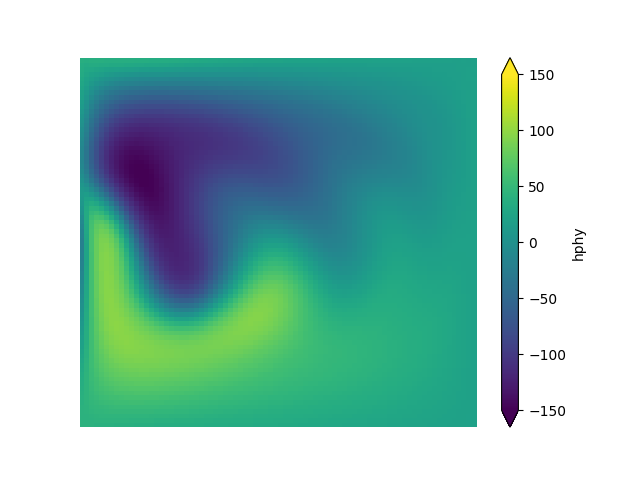
\includegraphics[width=\textwidth]{./fig/L3/mean-hphy0.png}\\
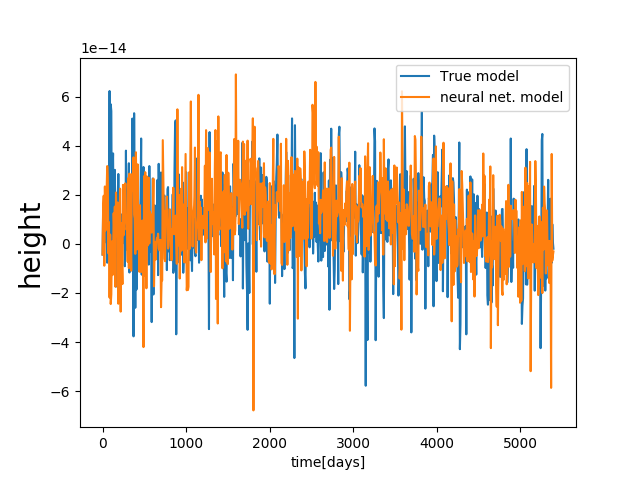
\includegraphics[width=\textwidth]{./fig/L3/evol-h.png}
\column{.3\textwidth}
\centering
{\footnotesize mean $h$ for nn model}\\
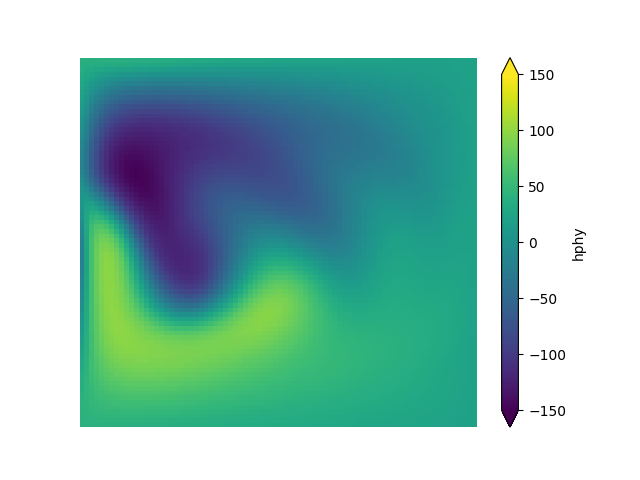
\includegraphics[width=\textwidth]{./fig/L3/mean-hphy1.png}\\
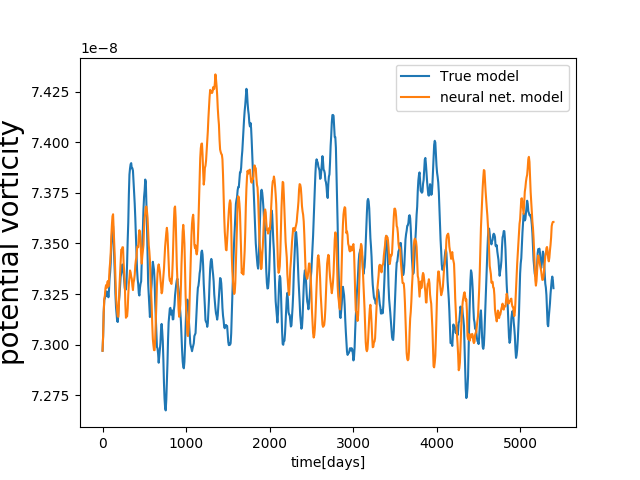
\includegraphics[width=\textwidth]{./fig/L3/evol-PV.png}
\column{.3\textwidth}
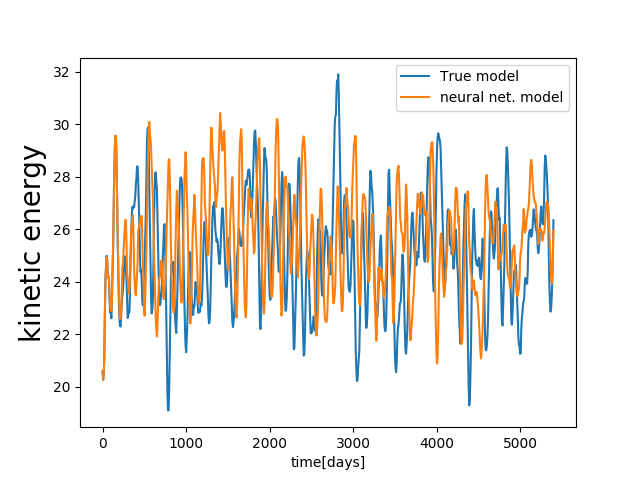
\includegraphics[width=\textwidth]{./fig/L3/evol-EC.png}\\
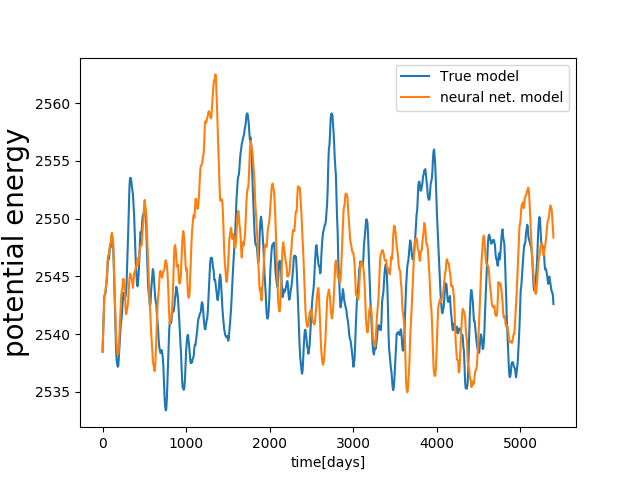
\includegraphics[width=\textwidth]{./fig/L3/evol-EP.png}
\end{columns}
\end{frame}

%%%%%%%%%%%%%%%%%%%%%%%
\begin{frame}
\frametitle{Generalization skills}
\frametitle{Simulation with a different wind forcing}
\begin{alertblock}{Objective}
Has the neural net learned systematic features or can it simulate something (relatively) new ?
\end{alertblock}
\pause
Idea : Try a neural net simulation with a new wind forcing.
\begin{figure}
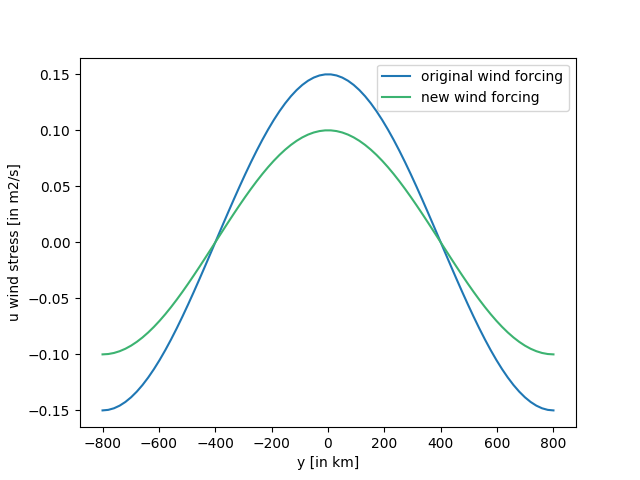
\includegraphics[width=.6\textwidth]{./fig/L3/wind_forcing.png}
\end{figure}
\end{frame}

%%%%%%%%%%%%%%%%%%%%%
\begin{frame}
\frametitle{Simulation with a different wind-forcing}
~\\
\begin{columns}
\column{.5\textwidth}
\centering
With the original wind-forcing
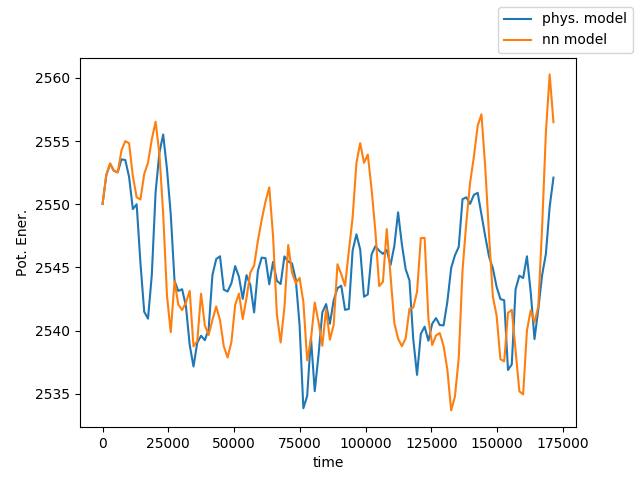
\includegraphics[width=\textwidth]{./fig/L3/Ep_std.png}\\
\column{.5\textwidth}
\centering
With the low wind-forcing
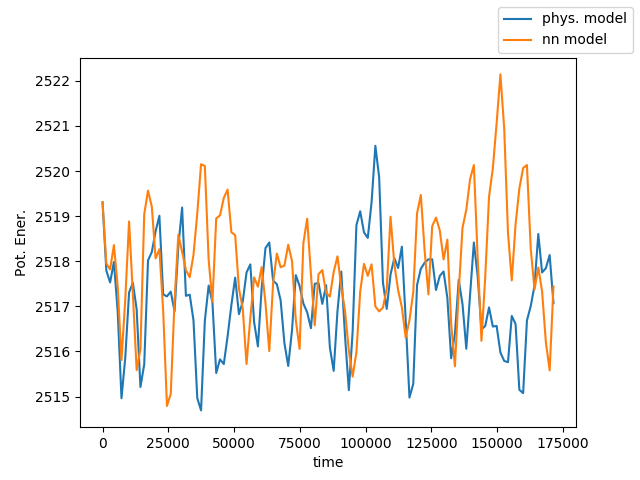
\includegraphics[width=\textwidth]{./fig/L3/Ep_windlow.png}\\
\end{columns}
\pause
\begin{table}
\footnotesize
\begin{tabular}{|r|c|c|c|c|}
\hline
& \multicolumn{2}{c|}{ref wind} & \multicolumn{2}{c|}{low wind} \\
\hline
P. E.  &$ 2545 \pm 2$ & $2545 \pm3$  &  $ 2517 \pm 1$ & $2518 \pm1$\\
K. E. & $25 \pm 1$& $25 \pm 1$ &$11.8 \pm 0.3$ & $12.0 \pm 0.4$\\
P. V. & $7.332 \pm 0.01$   & $7.339 \pm 0.02$ & $7.159 \pm 0.004 $ & $7.165 \pm 0.005 $ \\
\hline
\end{tabular}
\end{table}
\end{frame}

\begin{frame}{}
   \bibliography{references.bib}
\end{frame}
    
%%%%%%%%%%%%%%%%%%%%%
%%%%%%%%%%%%%%%%%%%%%
%%%%%%%%%%%%%%%%%%%%%
%%%%%%%%%%%%%%%%%%%%%
%%%%%%%%%%%%%%%%%%%%%%%%%%%%%%%%%%%%%%%%%%
%%%%%%%%%%%%%%%%%%%%%
%%%%%%%%%%%%%%%%%%%%%%%%%%%%%%%%%%%%%%%%%%
\end{document}
%%%%%%%%%%%%%%%%%%%%%%%%%%%%%%%%%%%%%%%%%%



